\documentclass[11pt]{beamer}

\usepackage{lmodern}
\usepackage[beamer,customcolors]{hf-tikz}

\tikzset{hl/.style={
    set fill color=red!80!black!40,
    set border color=red!80!black,
  },
}

\addtobeamertemplate{navigation symbols}{}{%
    \usebeamerfont{footline}%
    \usebeamercolor[fg]{footline}%
    \hspace{1em}%
    \insertframenumber/\inserttotalframenumber
}

\usetheme{Montpellier}
\usepackage[utf8]{inputenc}
\usepackage[english,american]{babel}
\usepackage{amsmath}
\usepackage{amsfonts}
\usepackage{amssymb}
\usepackage{graphicx}
\usepackage{booktabs}
\usepackage{float}
\usepackage{multirow}
\usepackage{subcaption}
\usepackage{threeparttable}
\usepackage{pdflscape}
\usepackage{lscape}
\usepackage{array}
\usepackage{tabulary}
\newcolumntype{K}[1]{>{\centering\arraybackslash}p{#1}}

	
\author[Francisco Cavalcanti]{Francisco Cavalcanti\\\footnotesize{PUC-Rio}
}

\author{
Gustavo Gonzaga \\
\textit{PUC-Rio}\\ \vspace{3mm}
\and  
Francisco Cavalcanti\\
\textit{PUC-Rio}\\ \vspace{3mm}
\and   
Flávia  Alfenas\\
\textit{Climate Policy Initiative (CPI)} 
}

\date{Junho, 2020}

\title{Mercado de Trabalho na Amazônia Legal}

\usepackage{tikz}
\def\checkmark{\tikz\fill[scale=0.4](0,.35) -- (.25,0) -- (1,.7) -- (.25,.15) -- cycle;} 


\newcommand{\quotes}[1]{``#1''}


\setbeamercovered{transparent} 
%\setbeamertemplate{navigation symbols}{} 
%\logo{} 
%\institute{} 
%\date{} 
%\subject{} 
\begin{document}

\begin{frame}
\titlepage
\end{frame}

%\begin{frame}
%\tableofcontents
%\end{frame}

\section{Introdução}

\begin{frame}[label=indice_principal]{Índice Principal}

\begin{itemize}
\item{
	\hyperlink{_estrutura_emprego}{\beamerbutton{Estrutrura do Emprego}} - Descreve a estrutura e evolução do emprego da Amazônia Legal e compara com o resto do Brasil.
	}   
		
\item{
	\hyperlink{_estrutura_renda}{\beamerbutton{Estrutura da Renda}} - Descreve a estrutura e evolução de rendimentos e desigualdade da Amazônia Legal e compara com o resto do Brasil.
	}  
	
\item{
	\hyperlink{_programas_sociais}{\beamerbutton{Programas Sociais}} - Descreve a presença de programas sociais na Amazônia Legal e compara com o resto do Brasil.
	}  
	
\item{
	\hyperlink{_transicao_ocupacao}{\beamerbutton{Transição de Ocupações}} - Descreve o risco associado a cada ocupação e como esse risco evoluiu ao longo do tempo para a Amazônia Legal e compara com o resto do Brasil.
	}  
	
\item{
	\hyperlink{_composicao_demografica}{\beamerbutton{Composição Demográfica}} - Esta seção destrincha a estrutura do mercado de trabalho na Amazônia Legal por composições demográficas.
	}  

\end{itemize}

\end{frame}

\section{Estrutura do Emprego}

\begin{frame}[label=_estrutura_emprego]{Estrutura do Emprego}
{\footnotesize Fonte de dados: Dados da PNAD Contínua Trimestral (2012-2020)}
\begin{itemize}
\item{Taxa de ocupação: \hyperlink{_estrutura_emprego_taxa_de_ocupacao}{\beamerbutton{clique aqui}}}
\item{Taxa de informalidade: \hyperlink{_estrutura_emprego_taxa_de_informalidade}{\beamerbutton{clique aqui}}}
\item{Taxa de desemprego: \hyperlink{_estrutura_emprego_taxa_de_desemprego}{\beamerbutton{clique aqui}}}
\item{Taxa de participação: \hyperlink{_estrutura_emprego_taxa_de_participacao}{\beamerbutton{clique aqui}}}
\item{Proporção de militares e estatutários: \hyperlink{_estrutura_emprego_prop_militar}{\beamerbutton{clique aqui}}}
\item{Proporção de empregados sem carteira: \hyperlink{_estrutura_emprego_prop_empregadoSC}{\beamerbutton{clique aqui}}}
\item{Proporção de empregados com carteira: \hyperlink{_estrutura_emprego_prop_empregadoCC}{\beamerbutton{clique aqui}}}
\item{Proporção de empregadores \hyperlink{_estrutura_emprego_prop_empregador}{\beamerbutton{clique aqui}}}
\item{Proporção de conta própria: \hyperlink{_estrutura_emprego_prop_cpropria}{\beamerbutton{clique aqui}}}
\item{Proporção de conta própria que contribui: \hyperlink{_estrutura_emprego_prop_cpropriaC}{\beamerbutton{clique aqui}}}
\item{Proporção de conta própria que não contribui: \hyperlink{_estrutura_emprego_prop_cpropriaNc}{\beamerbutton{clique aqui}}}
\end{itemize}

\begin{small}
\textit{Retornar ao índice principal: \hyperlink{indice_principal}{\beamerbutton{AQUI}} }
\end{small}

\end{frame}

\begin{frame}[label=_estrutura_emprego_taxa_de_ocupacao]{}
\textit{\hyperlink{_estrutura_emprego}{\beamerbutton{Voltar}}}
\begin{figure}
  \centering
  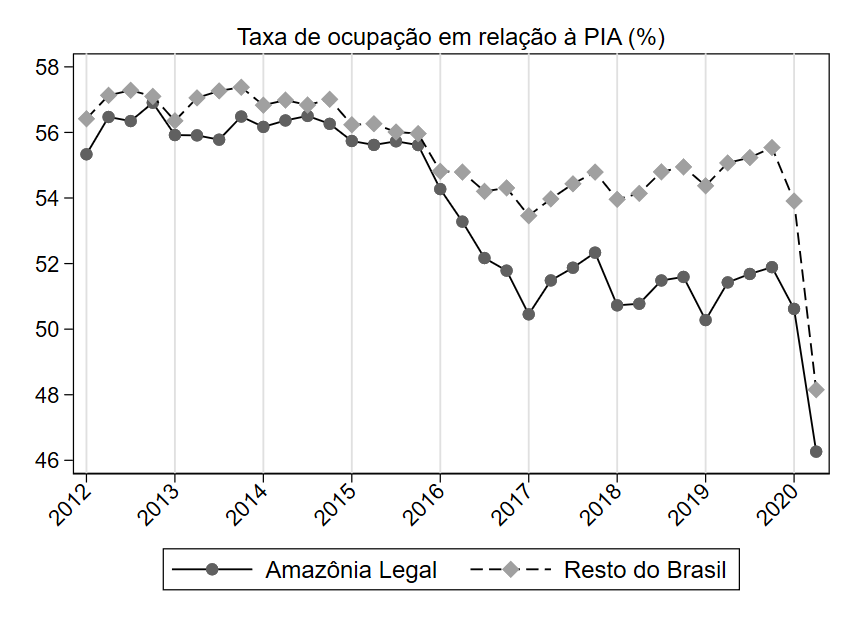
\includegraphics[width=1\linewidth]{../../analysis/output/estrutura_emprego/_estrutura_emprego_taxa_de_ocupacao.png}
  \caption{}
  \label{fig:_estrutura_emprego_taxa_de_ocupacao}
\end{figure}
\end{frame}

\begin{frame}[label=_estrutura_emprego_taxa_de_informalidade]{}
\textit{\hyperlink{_estrutura_emprego}{\beamerbutton{Voltar}}}
\begin{figure}
  \centering
  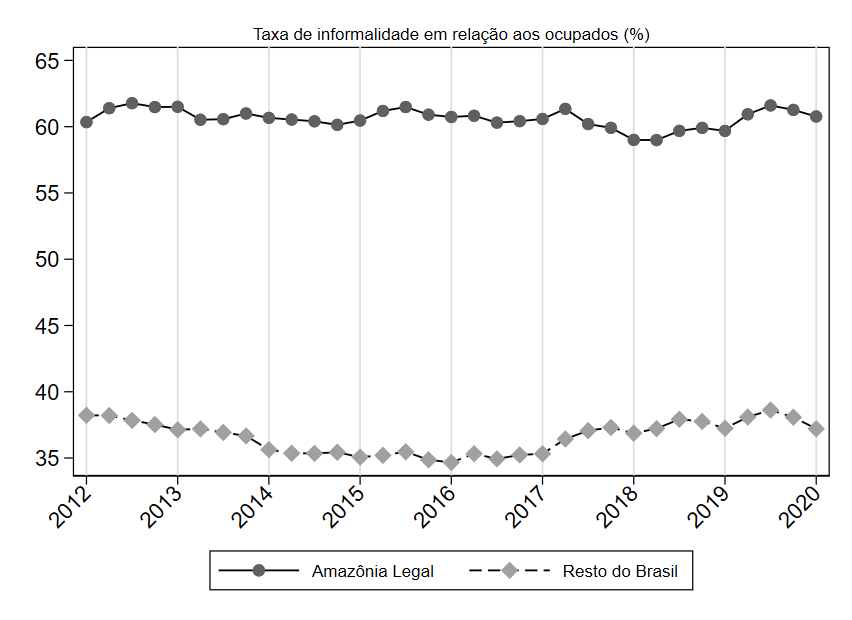
\includegraphics[width=1.0\linewidth]{../../analysis/output/estrutura_emprego/_estrutura_emprego_taxa_de_informalidade.png}
  \caption{}
  \label{fig:_estrutura_emprego_taxa_de_informalidade}
\end{figure}
\end{frame}

\begin{frame}[label=_estrutura_emprego_taxa_de_desemprego]{}
\textit{\hyperlink{_estrutura_emprego}{\beamerbutton{Voltar}}}
\begin{figure}
  \centering
  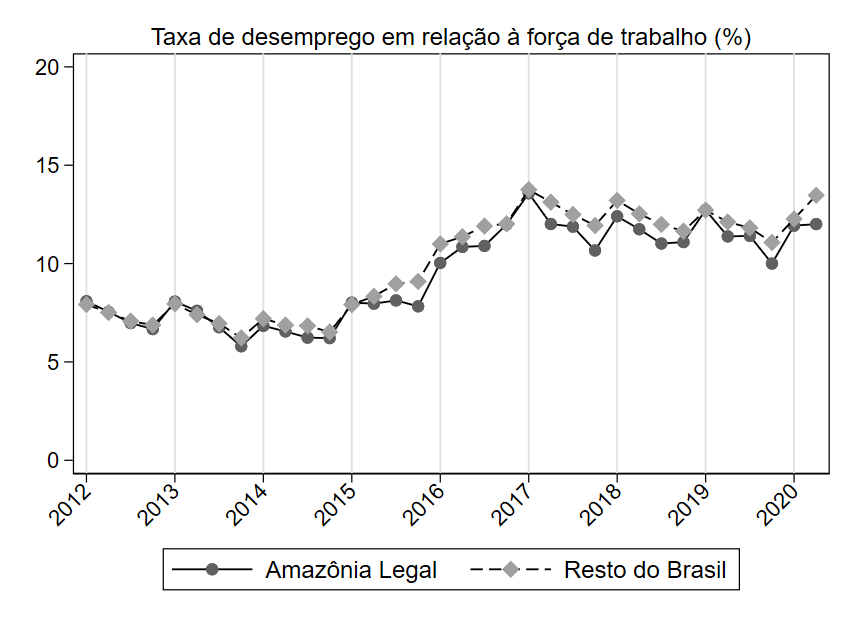
\includegraphics[width=1.0\linewidth]{../../analysis/output/estrutura_emprego/_estrutura_emprego_taxa_de_desemprego.png}
  \caption{}
  \label{fig:_estrutura_emprego_taxa_de_desemprego}
\end{figure}
\end{frame}

\begin{frame}[label=_estrutura_emprego_taxa_de_participacao]{}
\textit{\hyperlink{_estrutura_emprego}{\beamerbutton{Voltar}}}
\begin{figure}
  \centering
  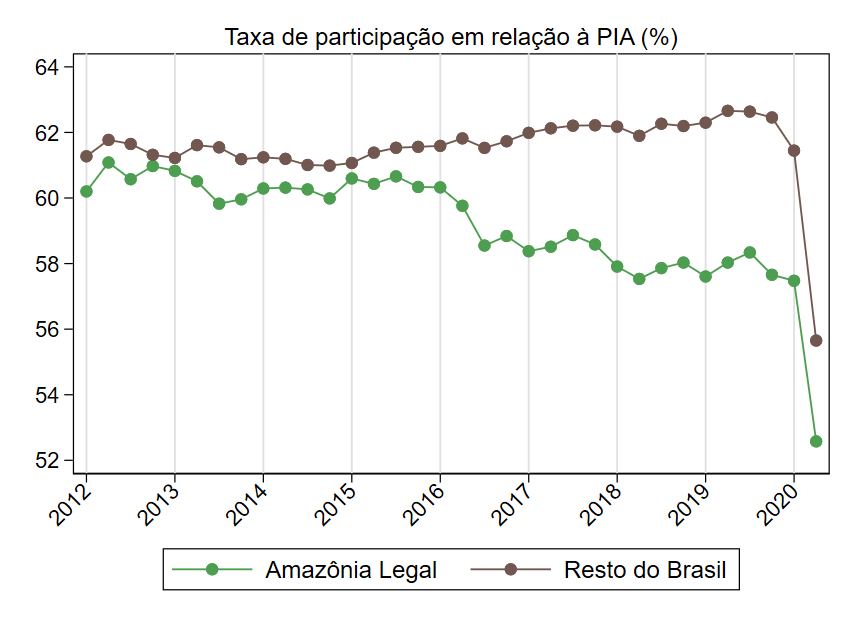
\includegraphics[width=1.0\linewidth]{../../analysis/output/estrutura_emprego/_estrutura_emprego_taxa_de_participacao.png}
  \caption{}
  \label{fig:_estrutura_emprego_taxa_de_participacao}
\end{figure}
\end{frame}


\begin{frame}[label=_estrutura_emprego_prop_militar]{}
\textit{\hyperlink{_estrutura_emprego}{\beamerbutton{Voltar}}}
\begin{figure}
  \centering
  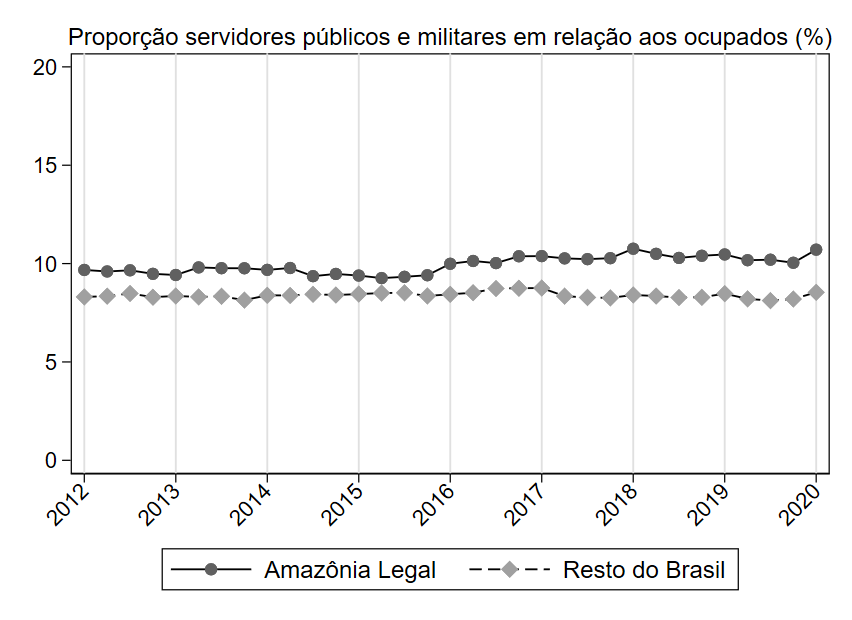
\includegraphics[width=1.0\linewidth]{../../analysis/output/estrutura_emprego/_estrutura_emprego_prop_militar.png}
  \caption{}
  \label{fig:_estrutura_emprego_prop_militar}
\end{figure}
\end{frame}


\begin{frame}[label=_estrutura_emprego_prop_empregadoSC]{}
\textit{\hyperlink{_estrutura_emprego}{\beamerbutton{Voltar}}}
\begin{figure}
  \centering
  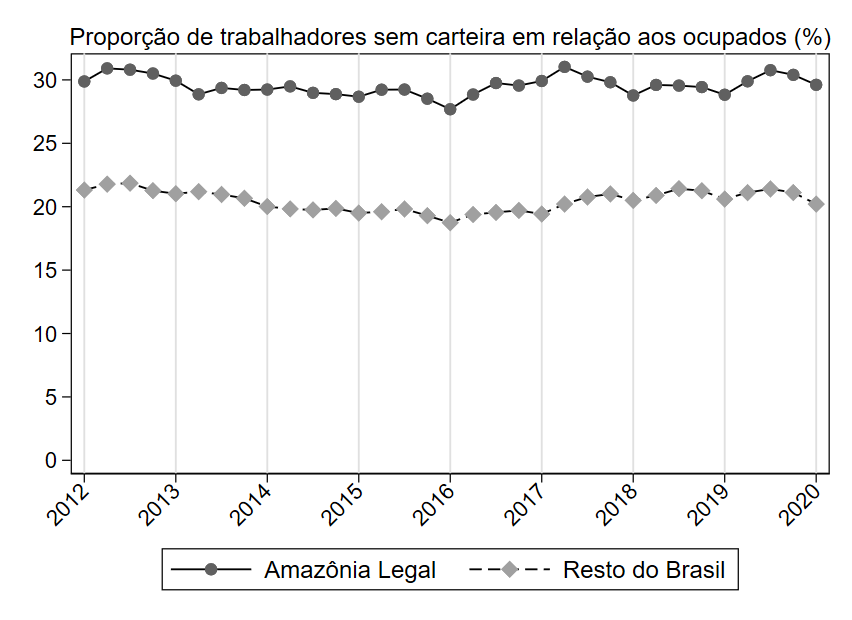
\includegraphics[width=1.0\linewidth]{../../analysis/output/estrutura_emprego/_estrutura_emprego_prop_empregadoSC.png}
  \caption{}
  \label{fig:_estrutura_emprego_prop_empregadoSC}
\end{figure}
\end{frame}

\begin{frame}[label=_estrutura_emprego_prop_empregadoCC]{}
\textit{\hyperlink{_estrutura_emprego}{\beamerbutton{Voltar}}}
\begin{figure}
  \centering
  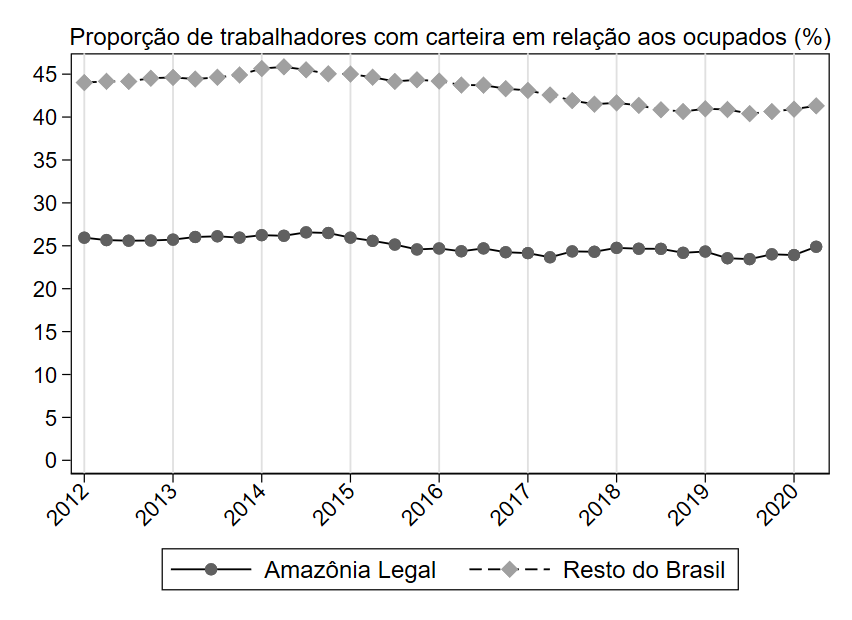
\includegraphics[width=1.0\linewidth]{../../analysis/output/estrutura_emprego/_estrutura_emprego_prop_empregadoCC.png}
  \caption{}
  \label{fig:_estrutura_emprego_prop_empregadoCC}
\end{figure}
\end{frame}

\begin{frame}[label=_estrutura_emprego_prop_empregador]{}
\textit{\hyperlink{_estrutura_emprego}{\beamerbutton{Voltar}}}
\begin{figure}
  \centering
  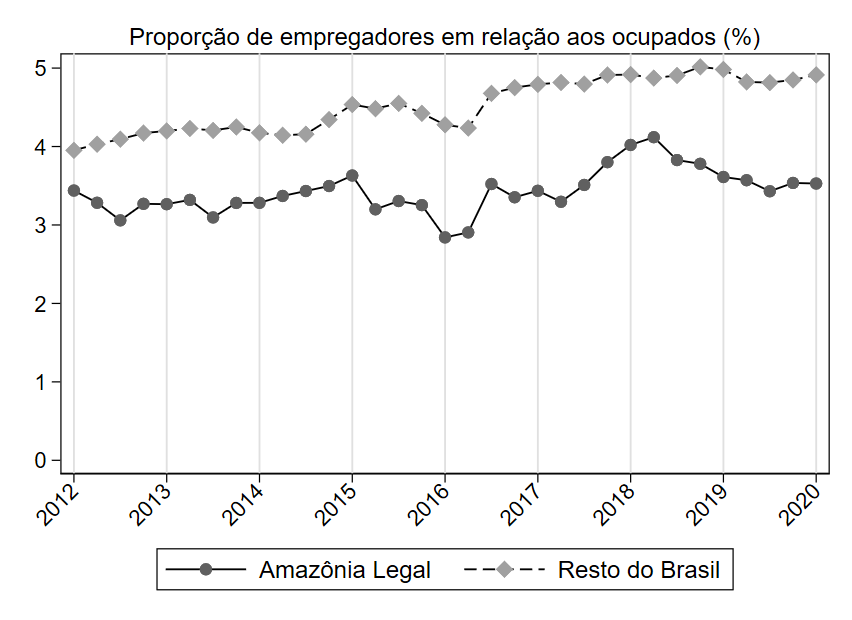
\includegraphics[width=1.0\linewidth]{../../analysis/output/estrutura_emprego/_estrutura_emprego_prop_empregador.png}
  \caption{}
  \label{fig:_estrutura_emprego_prop_empregador}
\end{figure}
\end{frame}



\begin{frame}[label=_estrutura_emprego_prop_cpropria]{}
\textit{\hyperlink{_estrutura_emprego}{\beamerbutton{Voltar}}}
\begin{figure}
  \centering
  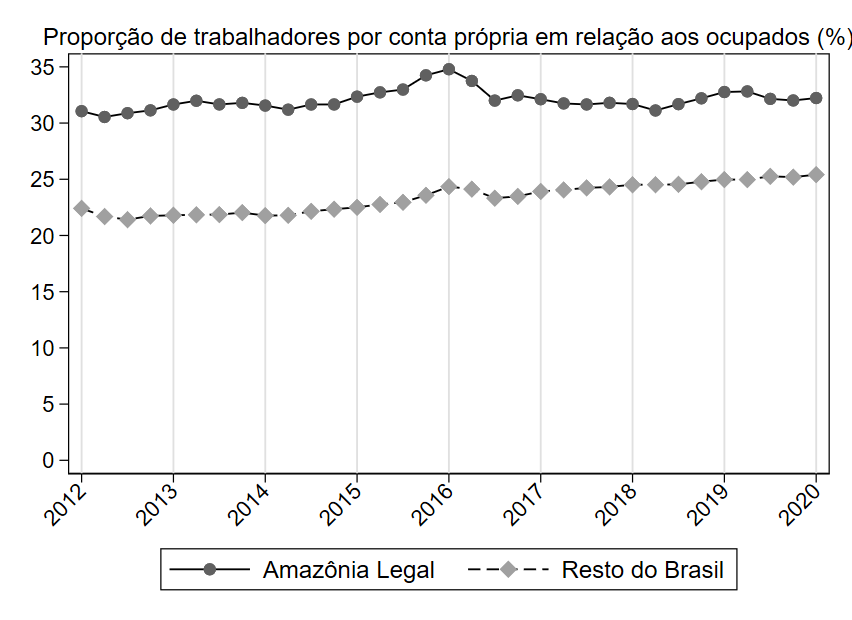
\includegraphics[width=1.0\linewidth]{../../analysis/output/estrutura_emprego/_estrutura_emprego_prop_cpropria.png}
  \caption{}
  \label{fig:_estrutura_emprego_prop_cpropria}
\end{figure}
\end{frame}

\begin{frame}[label=_estrutura_emprego_prop_cpropriaC]{}
\textit{\hyperlink{_estrutura_emprego}{\beamerbutton{Voltar}}}
\begin{figure}
  \centering
  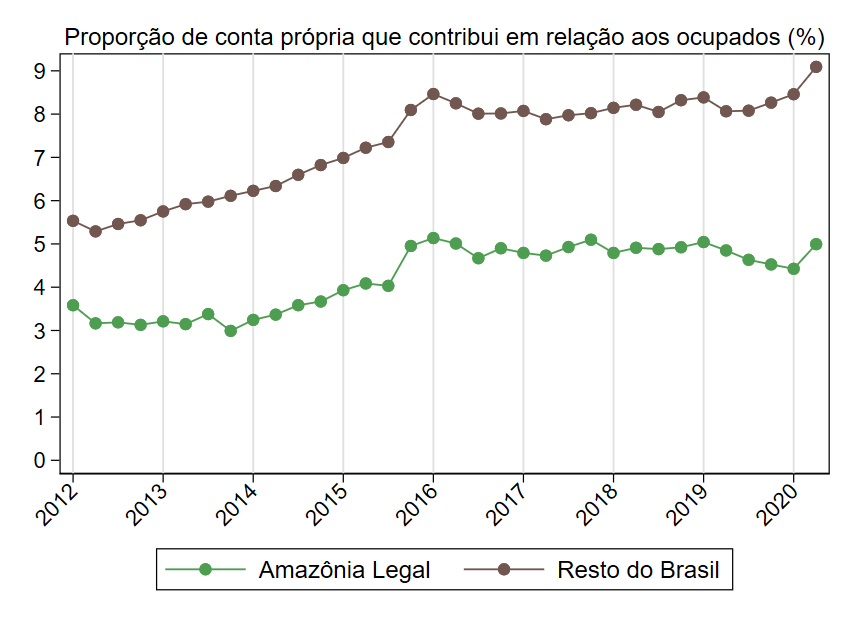
\includegraphics[width=1.0\linewidth]{../../analysis/output/estrutura_emprego/_estrutura_emprego_prop_cpropriaC.png}
  \caption{}
  \label{fig:_estrutura_emprego_prop_cpropriaC}
\end{figure}
\end{frame}

\begin{frame}[label=_estrutura_emprego_prop_cpropriaNc]{}
\textit{\hyperlink{_estrutura_emprego}{\beamerbutton{Voltar}}}
\begin{figure}
  \centering
  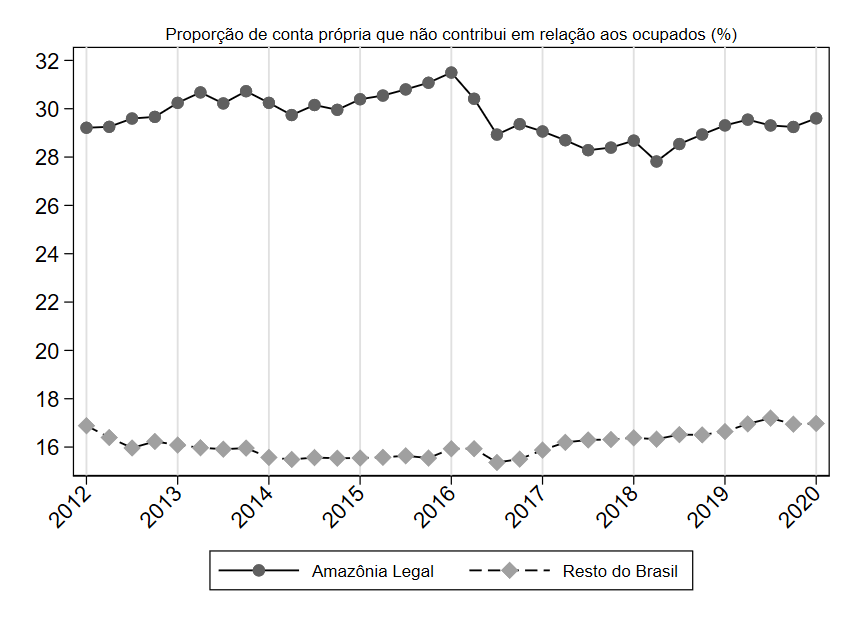
\includegraphics[width=1.0\linewidth]{../../analysis/output/estrutura_emprego/_estrutura_emprego_prop_cpropriaNc.png}
  \caption{}
  \label{fig:_estrutura_emprego_prop_cpropriaNc}
\end{figure}
\end{frame}

\section{Estrutura da Renda}

\begin{frame}[label=_estrutura_renda]{Estrutura da Renda}
{\footnotesize Fonte de dados: Dados da PNAD Contínua Trimestral (2012-2020)}
\begin{footnotesize}
\begin{itemize}
\item{Rendimento médio: \hyperlink{_estrutura_renda_rendimento_medio_total}{\beamerbutton{clique aqui}}}
\item{Rendimento médio no setor informal: \hyperlink{_estrutura_renda_rendimento_medio_informal}{\beamerbutton{clique aqui}}}
\item{Rendimento médio no setor formal: \hyperlink{_estrutura_renda_rendimento_medio_formal}{\beamerbutton{clique aqui}}}
\item{Rendimento domiciliar per capita: \hyperlink{_estrutura_renda_rendimento_domiciliar_pc}{\beamerbutton{clique aqui}}}

\item{Proporção de indivíduos com renda mensal domiciliar per capita de até 300,00 Reais: \hyperlink{_estrutura_renda_prop_rendimento_domiciliar_BF}{\beamerbutton{clique aqui}}}

\item{GINI dominciliar per capita: \hyperlink{_estrutura_renda_gini_rendimento_domiciliar_pc}{\beamerbutton{clique aqui}}}
\item{GINI dos ocupados: \hyperlink{_estrutura_renda_gini_ocupado}{\beamerbutton{clique aqui}}}
\item{GINI dos informais \hyperlink{_estrutura_renda_gini_informal}{\beamerbutton{clique aqui}}}
\item{GINI dos formais \hyperlink{_estrutura_renda_gini_formal}{\beamerbutton{clique aqui}}}
\end{itemize}
\end{footnotesize}

\begin{small}
\textit{Retornar ao índice principal: \hyperlink{indice_principal}{\beamerbutton{AQUI}} }
\end{small}

\end{frame}

\begin{frame}[label=_estrutura_renda_rendimento_medio_total]{}
\textit{\hyperlink{_estrutura_renda}{\beamerbutton{Voltar}}}
\begin{figure}
  \centering
  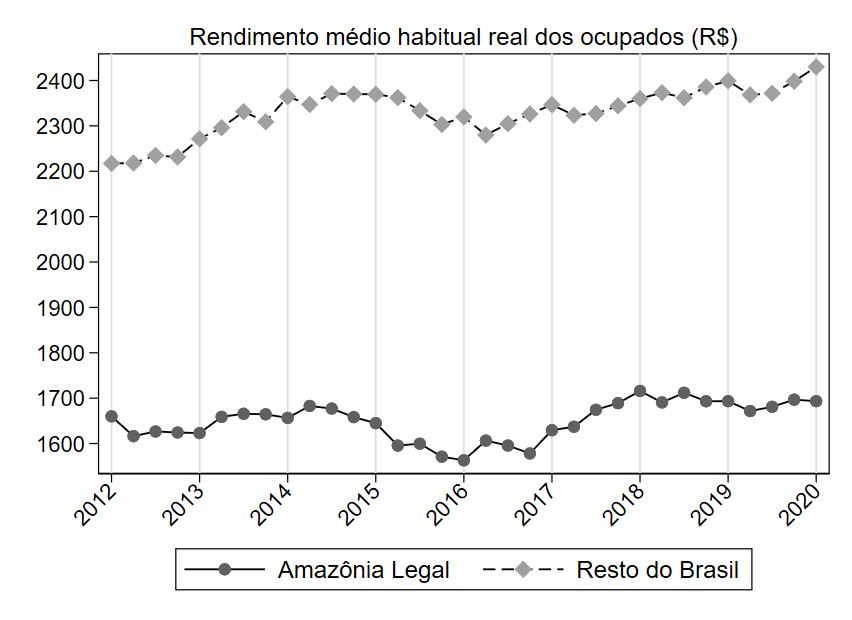
\includegraphics[width=1\linewidth]{../../analysis/output/estrutura_renda/_estrutura_renda_rendimento_medio_total.png}
  \caption{}
  \label{fig:_estrutura_renda_rendimento_medio_total}
\end{figure}
\end{frame}

\begin{frame}[label=_estrutura_renda_rendimento_medio_informal]{}
\textit{\hyperlink{_estrutura_renda}{\beamerbutton{Voltar}}}
\begin{figure}
  \centering
  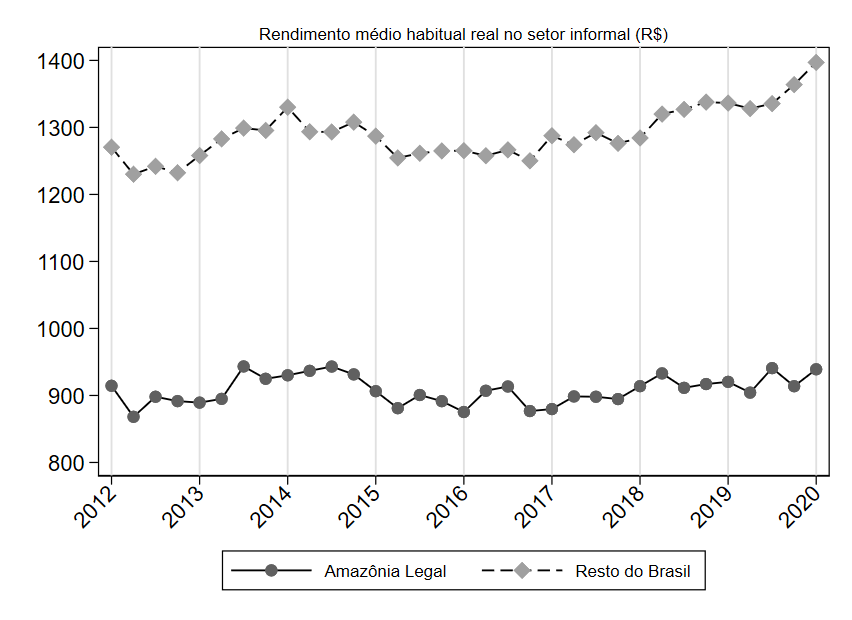
\includegraphics[width=1.0\linewidth]{../../analysis/output/estrutura_renda/_estrutura_renda_rendimento_medio_informal.png}
  \caption{}
  \label{fig:_estrutura_renda_rendimento_medio_informal}
\end{figure}
\end{frame}

\begin{frame}[label=_estrutura_renda_rendimento_medio_formal]{}
\textit{\hyperlink{_estrutura_renda}{\beamerbutton{Voltar}}}
\begin{figure}
  \centering
  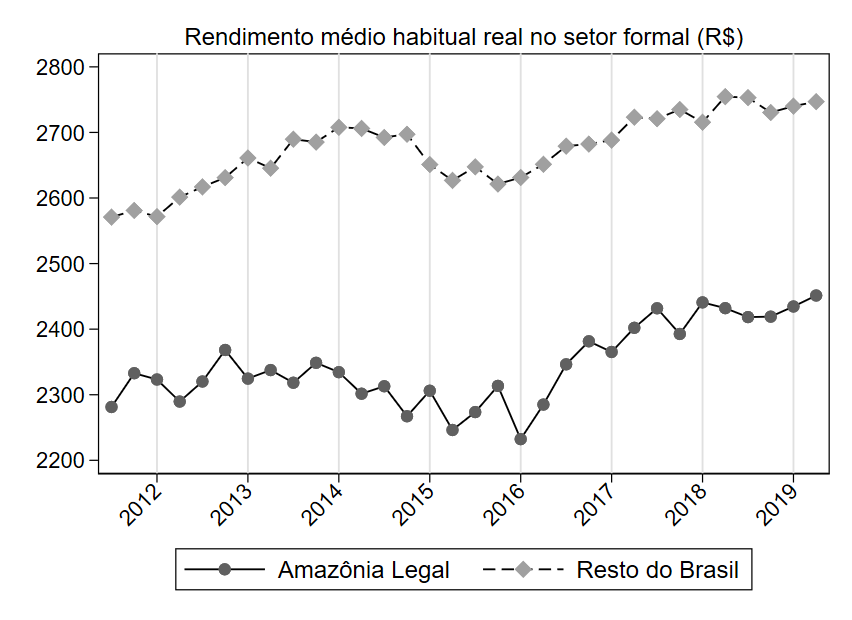
\includegraphics[width=1.0\linewidth]{../../analysis/output/estrutura_renda/_estrutura_renda_rendimento_medio_formal.png}
  \caption{}
  \label{fig:_estrutura_renda_rendimento_medio_formal}
\end{figure}
\end{frame}

\begin{frame}[label=_estrutura_renda_rendimento_domiciliar_pc]{}
\textit{\hyperlink{_estrutura_renda}{\beamerbutton{Voltar}}}
\begin{figure}
  \centering
  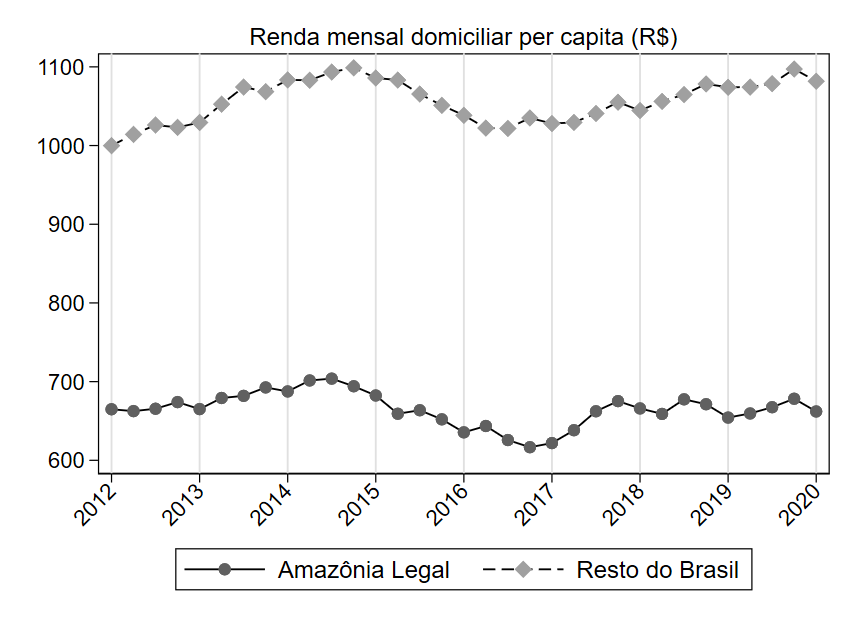
\includegraphics[width=1.0\linewidth]{../../analysis/output/estrutura_renda/_estrutura_renda_rendimento_domiciliar_pc.png}
  \caption{}
  \label{fig:_estrutura_renda_rendimento_domiciliar_pc}
\end{figure}
\end{frame}


\begin{frame}[label=_estrutura_renda_prop_rendimento_domiciliar_BF]{}
\textit{\hyperlink{_estrutura_renda}{\beamerbutton{Voltar}}}
\begin{figure}
  \centering
  \includegraphics[width=1.0\linewidth]{../../analysis/output/estrutura_renda/_estrutura_renda_prop_rendimento_domiciliar_BF.png}
  \caption{}
  \label{fig:_estrutura_renda_prop_rendimento_domiciliar_BF}
\end{figure}
\end{frame}

\begin{frame}[label=_estrutura_renda_gini_rendimento_domiciliar_pc]{}
\textit{\hyperlink{_estrutura_renda}{\beamerbutton{Voltar}}}
\begin{figure}
  \centering
  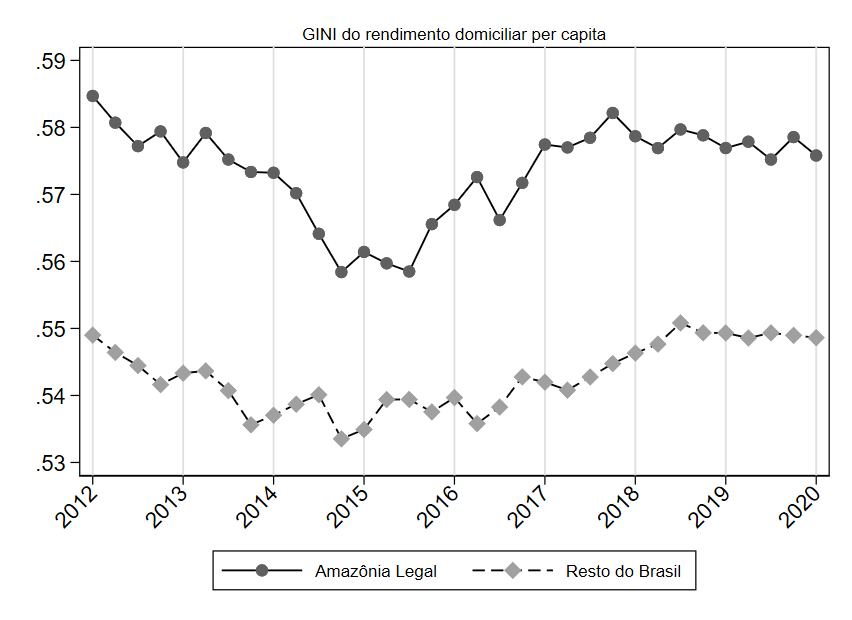
\includegraphics[width=1.0\linewidth]{../../analysis/output/estrutura_renda/_estrutura_renda_gini_rendimento_domiciliar_pc.png}
  \caption{}
  \label{fig:_estrutura_renda_gini_rendimento_domiciliar_pc}
\end{figure}
\end{frame}

\begin{frame}[label=_estrutura_renda_gini_ocupado]{}
\textit{\hyperlink{_estrutura_renda}{\beamerbutton{Voltar}}}
\begin{figure}
  \centering
  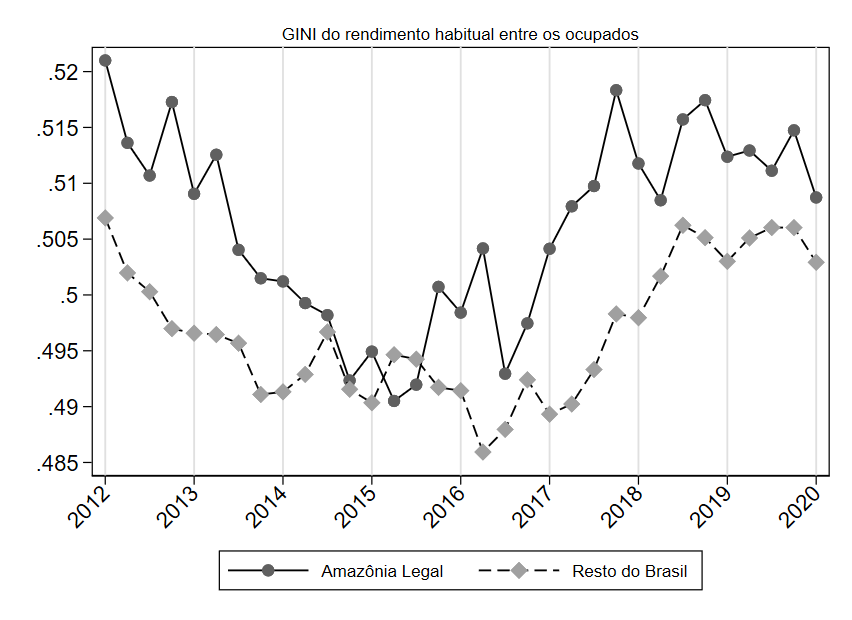
\includegraphics[width=1.0\linewidth]{../../analysis/output/estrutura_renda/_estrutura_renda_gini_ocupado.png}
  \caption{}
  \label{fig:_estrutura_renda_gini_ocupado}
\end{figure}
\end{frame}

\begin{frame}[label=_estrutura_renda_gini_informal]{}
\textit{\hyperlink{_estrutura_renda}{\beamerbutton{Voltar}}}
\begin{figure}
  \centering
  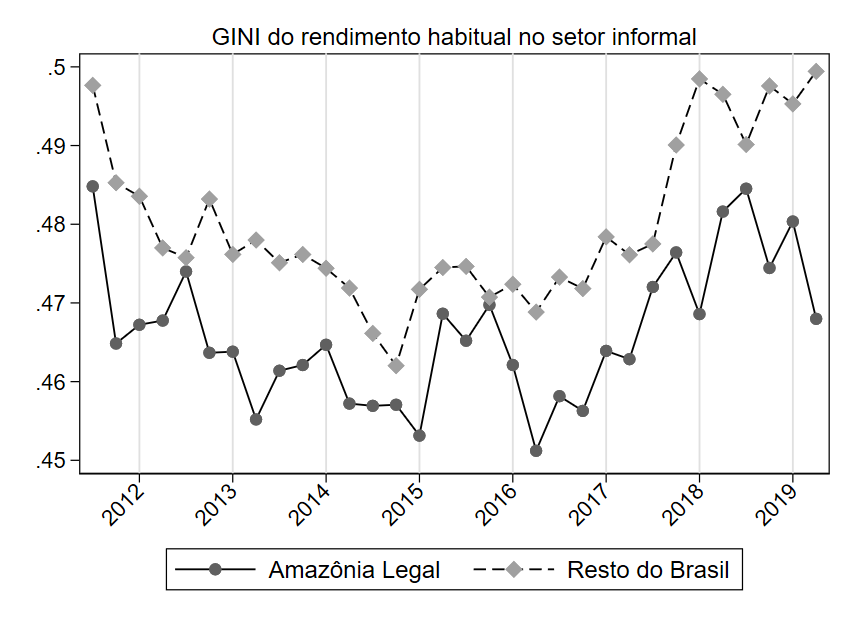
\includegraphics[width=1.0\linewidth]{../../analysis/output/estrutura_renda/_estrutura_renda_gini_informal.png}
  \caption{}
  \label{fig:_estrutura_renda_gini_informal}
\end{figure}
\end{frame}


\begin{frame}[label=_estrutura_renda_gini_formal]{}
\textit{\hyperlink{_estrutura_renda}{\beamerbutton{Voltar}}}
\begin{figure}
  \centering
  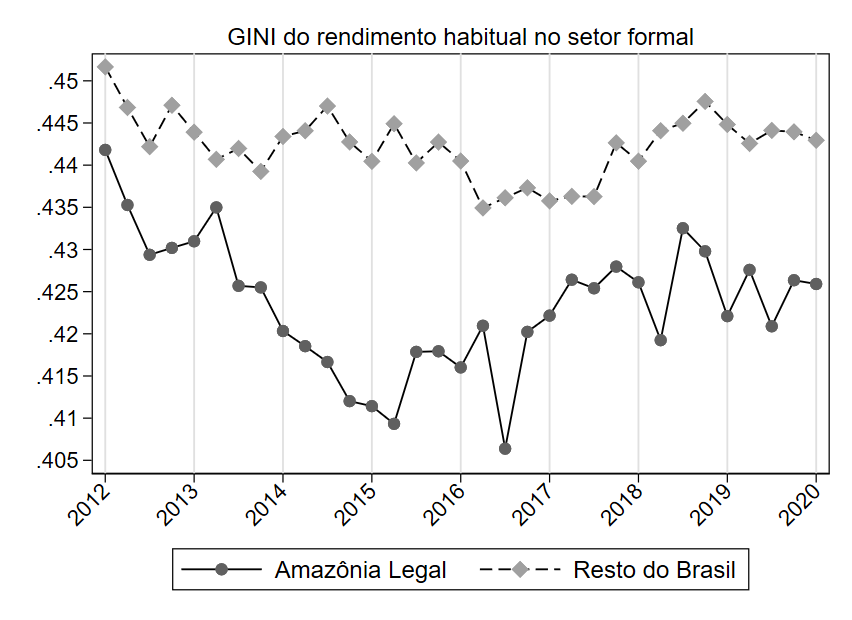
\includegraphics[width=1.0\linewidth]{../../analysis/output/estrutura_renda/_estrutura_renda_gini_formal.png}
  \caption{}
  \label{fig:_estrutura_renda_gini_formal}
\end{figure}
\end{frame}


\section{Programas Sociais}

\begin{frame}[label=_programas_sociais]{Programas Sociais}
{\footnotesize Fonte de dados: Dados da PNAD Contínua Anual (2012-2019)}
\begin{itemize}
\item{Proporção da população que benificiária de programas sociais \hyperlink{_programas_sociais_prop_ajuda_gov}{\beamerbutton{clique aqui}}}
\item{Proporção da população que benificiária de Bolsa Família  \hyperlink{_programas_sociais_prop_bolsa_familia}{\beamerbutton{clique aqui}}}
\item{Proporção da população que benificiária de BPC-LOAS  \hyperlink{_programas_sociais_prop_bpc_loas}{\beamerbutton{clique aqui}}}
\end{itemize}

\begin{small}
\textit{Retornar ao índice principal: \hyperlink{indice_principal}{\beamerbutton{AQUI}} }
\end{small}

\end{frame}

\begin{frame}[label=_programas_sociais_prop_ajuda_gov]{}
\textit{\hyperlink{_programas_sociais}{\beamerbutton{Voltar}}}
\begin{figure}
  \centering
  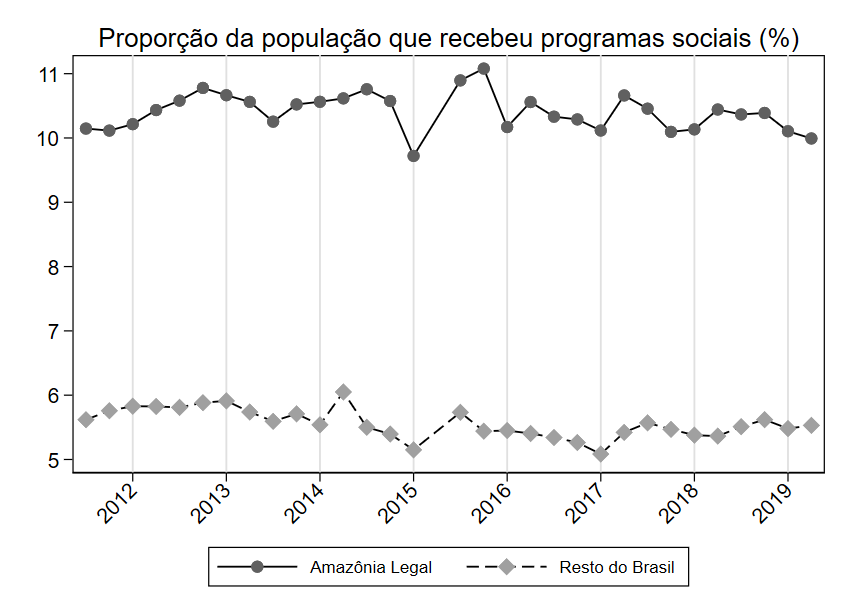
\includegraphics[width=1\linewidth]{../../analysis/output/programas_sociais/_programas_sociais_prop_ajuda_gov.png}
  \caption{}
  \label{fig:_programas_sociais_prop_ajuda_gov}
\end{figure}
\end{frame}

\begin{frame}[label=_programas_sociais_prop_bolsa_familia]{}
\textit{\hyperlink{_programas_sociais}{\beamerbutton{Voltar}}}
\begin{figure}
  \centering
  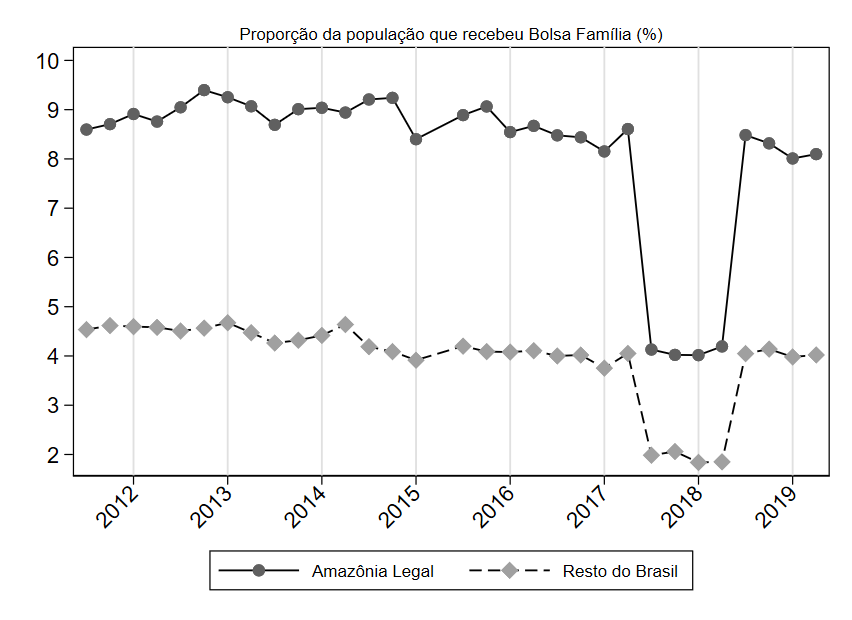
\includegraphics[width=1.0\linewidth]{../../analysis/output/programas_sociais/_programas_sociais_prop_bolsa_familia.png}
  \caption{}
  \label{fig:_programas_sociais_prop_bolsa_familia}
\end{figure}
\end{frame}

\begin{frame}[label=_programas_sociais_prop_bpc_loas]{}
\textit{\hyperlink{_programas_sociais}{\beamerbutton{Voltar}}}
\begin{figure}
  \centering
  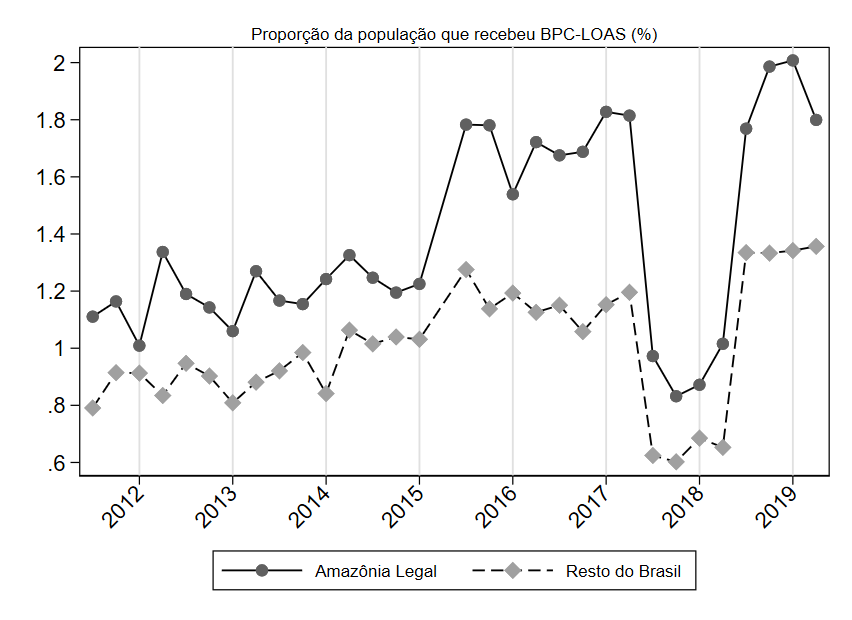
\includegraphics[width=1.0\linewidth]{../../analysis/output/programas_sociais/_programas_sociais_prop_bpc_loas.png}
  \caption{}
  \label{fig:_programas_sociais_prop_bpc_loas}
\end{figure}
\end{frame}


\section{Transição de Ocupações}

\begin{frame}[label=_transicao_ocupacao]{Transição de Ocupações}
{\footnotesize Fonte de dados: Dados da PNAD Contínua Trimestral (2012-2020)}
\begin{itemize}

\item{Matriz de transição para Amazônia Legal: \hyperlink{_transicao_ocupacao_amazonia_legal_matriz}{\beamerbutton{clique aqui}}}

\item{Matriz de transição para o resto do Brasil: \hyperlink{_transicao_ocupacao_resto_brasil_matriz}{\beamerbutton{clique aqui}}}

\item{Diferença entre matrizes de transição: \hyperlink{_transicao_ocupacao_matriz_diferenca}{\beamerbutton{clique aqui}}}

\item{Transição de desempregado para formal: \hyperlink{_transicao_ocupacao_sh_desempregado_sh_formal}{\beamerbutton{clique aqui}}}
\item{Transição de desempregado para informal: \hyperlink{_transicao_ocupacao_sh_desempregado_sh_informal}{\beamerbutton{clique aqui}}}
\item{Transição de desempregado para inativa: \hyperlink{_transicao_ocupacao_sh_desempregado_sh_inativa}{\beamerbutton{clique aqui}}}
\item{Transição de formal para desempregado: \hyperlink{_transicao_ocupacao_sh_formal_sh_desempregado}{\beamerbutton{clique aqui}}}
\item{Transição de formal para inativa: \hyperlink{_transicao_ocupacao_sh_formal_sh_inativa}{\beamerbutton{clique aqui}}}
\item{Transição de formal para informal: \hyperlink{_transicao_ocupacao_sh_formal_sh_informal}{\beamerbutton{clique aqui}}}
\item{Transição de informal para desempregado: \hyperlink{_transicao_ocupacao_sh_informal_sh_desempregado}{\beamerbutton{clique aqui}}}
\item{Transição de informal para formal: \hyperlink{_transicao_ocupacao_sh_informal_sh_formal}{\beamerbutton{clique aqui}}}
\item{Transição de informal para inativa: \hyperlink{_transicao_ocupacao_sh_informal_sh_inativa}{\beamerbutton{clique aqui}}}

\end{itemize}

\begin{small}
\textit{Retornar ao índice principal: \hyperlink{indice_principal}{\beamerbutton{AQUI}} }
\end{small}

\end{frame}

\begin{frame}[label=_transicao_ocupacao_amazonia_legal_matriz]{}
\textit{\hyperlink{_transicao_ocupacao}{\beamerbutton{Voltar}}}
% Table generated by Excel2LaTeX from sheet 'Resto Brasil'
\begin{table}[htbp]
  \centering
  \caption{Matriz de transições trimestrais de posição da ocupação na Amazônia Legal em (\%)}
  	\scalebox{0.35}{  
		\begin{tabular}{lccccccccccc}
		\hline \hline
		&	\multicolumn{11}{c}{Trimestre subsequente} \\
		\hline \hline    
    	Trimestre anterior & Inativo & Desempregado & Trabalhador   & Trabalhador   & Empregado   & 	Empregado   & Conta   & Conta Própria   & Conta Própria   & Empregador & Militar e   \\
    	
    	  &   &   &   formal &   informal &   SC & 	  CC &   Própria &   que contribui &   que não contribui &   &   estatutário \\
		\\  	
    Inativo & 81.31 & 4.88  & 1.59  & 12.00 & 6.67  & 0.92  & 5.74  & 0.41  & 5.33  & 0.18  & 0.26 \\
    Desempregado & 33.58 & 33.24 & 7.09  & 25.80 & 15.75 & 6.23  & 10.56 & 0.51  & 10.05 & 0.28  & 0.35 \\
    Trabalhador formal & 4.58  & 2.14  & 79.17 & 13.13 & 7.60  & 49.27 & 9.71  & 4.19  & 5.52  & 0.99  & 25.71 \\
    Trabalhador informal & 15.58 & 4.14  & 8.32  & 70.46 & 33.81 & 4.11  & 39.36 & 2.71  & 36.65 & 1.49  & 1.50 \\
    Empregado SC & 16.82 & 5.01  & 10.16 & 67.24 & 57.03 & 6.42  & 11.19 & 0.97  & 10.21 & 0.76  & 2.77 \\
    Empregado CC & 4.76  & 3.09  & 81.72 & 9.97  & 7.54  & 79.19 & 2.91  & 0.48  & 2.44  & 0.46  & 2.06 \\
    Conta Própria & 13.79 & 3.05  & 10.11 & 70.37 & 10.00 & 1.84  & 68.35 & 7.99  & 60.36 & 2.68  & 0.28 \\
    Conta Própria que contribui & 9.58  & 1.44  & 38.86 & 43.92 & 7.98  & 2.43  & 71.50 & 35.55 & 35.94 & 6.20  & 0.87 \\
    Conta Própria que não contribui & 14.33 & 3.26  & 6.44  & 73.74 & 10.26 & 1.76  & 67.95 & 4.48  & 63.48 & 2.23  & 0.21 \\
    Empregador & 4.65  & 1.22  & 11.04 & 28.43 & 6.99  & 3.14  & 28.73 & 7.29  & 21.44 & 54.66 & 0.61 \\
    Militar e estatutário & 2.33  & 0.42  & 88.83 & 8.25  & 7.61  & 4.21  & 0.91  & 0.27  & 0.64  & 0.16  & 84.36 \\
    	\\
    	\hline \hline   
    	\end{tabular}%
    }	
  \label{tab:_transicao_ocupacao_resto_brasil_matriz}%
\end{table}%

\end{frame}

\begin{frame}[label=_transicao_ocupacao_resto_brasil_matriz]{}
\textit{\hyperlink{_transicao_ocupacao}{\beamerbutton{Voltar}}}
% Table generated by Excel2LaTeX from sheet 'Resto Brasil'
\begin{table}[htbp]
  \centering
  \caption{Matriz de transições trimestrais de posição da ocupação  no resto do Brasil em (\%)}
  	\scalebox{0.35}{  
		\begin{tabular}{lccccccccccc}
		\hline \hline
		&	\multicolumn{11}{c}{Trimestre subsequente} \\
		\hline \hline    
    	Trimestre anterior & Inativo & Desempregado & Trabalhador   & Trabalhador   & Empregado   & 	Empregado   & Conta   & Conta Própria   & Conta Própria   & Empregador & Militar e   \\
    	
    	  &   &   &   formal &   informal &   SC & 	  CC &   Própria &   que contribui &   que não contribui &   &   estatutário \\
		\\  	
    	Inativo & 86.64 & 4.47  & 2.20  & 6.51  & 3.80  & 1.54  & 3.18  & 0.47  & 2.71  & 0.15  & 0.19 \\
    	Desempregado & 25.61 & 43.75 & 11.24 & 19.17 & 12.37 & 10.02 & 7.73  & 0.93  & 6.80  & 0.23  & 0.29 \\
    	Trabalhador formal & 3.32  & 2.07  & 85.70 & 7.77  & 4.48  & 64.14 & 11.26 & 7.96  & 3.30  & 1.14  & 13.60 \\
    	Trabalhador informal & 12.00 & 4.94  & 14.00 & 67.55 & 36.76 & 7.80  & 35.95 & 5.16  & 30.79 & 1.50  & 1.04 \\
    	Empregado SC & 12.15 & 5.71  & 15.34 & 65.84 & 58.48 & 11.32 & 9.63  & 2.27  & 7.37  & 0.95  & 1.76 \\
    	Empregado CC & 3.30  & 2.53  & 88.14 & 5.61  & 4.35  & 85.73 & 1.96  & 0.70  & 1.26  & 0.43  & 1.71 \\
    	Conta Própria & 9.66  & 3.15  & 28.28 & 55.42 & 8.24  & 3.56  & 71.69 & 24.51 & 47.18 & 3.50  & 0.20 \\
    	Conta Própria que contribui & 4.96  & 1.35  & 62.92 & 24.42 & 5.89  & 3.99  & 77.12 & 58.59 & 18.53 & 6.34  & 0.35 \\
    	Conta Própria que não contribui & 11.82 & 3.98  & 12.31 & 69.70 & 9.32  & 3.36  & 69.19 & 8.81  & 60.38 & 2.19  & 0.13 \\
    	Empregador & 2.59  & 0.55  & 14.64 & 11.96 & 4.08  & 4.02  & 18.17 & 10.29 & 7.88  & 70.26 & 0.33 \\
    	Militar e estatutário & 2.00  & 0.38  & 93.31 & 4.14  & 3.87  & 8.23  & 0.58  & 0.31  & 0.27  & 0.18  & 84.77 \\
    	\\
    	\hline \hline   
    	\end{tabular}%
    }	
  \label{tab:_transicao_ocupacao_resto_brasil_matriz}%
\end{table}%

\end{frame}

\begin{frame}[label=_transicao_ocupacao_matriz_diferenca]{}
\textit{\hyperlink{_transicao_ocupacao}{\beamerbutton{Voltar}}}
% Table generated by Excel2LaTeX from sheet 'Resto Brasil'
\begin{table}[htbp]
  \centering
  \caption{Diferença entre as matrizes de transições trimestrais de posição da ocupação entre Amazônia Legal e o resto do Brasil em (\%)}
  	\scalebox{0.35}{  
		\begin{tabular}{lccccccccccc}
		\hline \hline
		&	\multicolumn{11}{c}{Trimestre subsequente} \\
		\hline \hline    
    	Trimestre anterior & Inativo & Desempregado & Trabalhador   & Trabalhador   & Empregado   & 	Empregado   & Conta   & Conta Própria   & Conta Própria   & Empregador & Militar e   \\
    	
    	  &   &   &   formal &   informal &   SC & 	  CC &   Própria &   que contribui &   que não contribui &   &   estatutário \\
		\\  	
    Inativo & -5.33 & 0.41  & -0.61 & 5.49  & 2.87  & -0.62 & 2.56  & -0.06 & 2.62  & 0.02  & 0.07 \\
    Desempregado & 7.98  & -10.51 & -4.15 & 6.63  & 3.38  & -3.79 & 2.84  & -0.42 & 3.25  & 0.05  & 0.06 \\
    Trabalhador formal & 1.26  & 0.07  & -6.54 & 5.35  & 3.13  & -14.88 & -1.55 & -3.77 & 2.22  & -0.15 & 12.11 \\
    Trabalhador informal & 3.58  & -0.80 & -5.69 & 2.92  & -2.94 & -3.69 & 3.41  & -2.45 & 5.86  & -0.01 & 0.45 \\
    Empregado SC & 4.67  & -0.69 & -5.19 & 1.40  & -1.45 & -4.90 & 1.55  & -1.29 & 2.85  & -0.19 & 1.00 \\
    Empregado CC & 1.46  & 0.56  & -6.42 & 4.37  & 3.19  & -6.54 & 0.96  & -0.22 & 1.18  & 0.03  & 0.34 \\
    Conta Própria & 4.13  & -0.10 & -18.17 & 14.95 & 1.76  & -1.72 & -3.34 & -16.53 & 13.19 & -0.82 & 0.08 \\
    Conta Própria que contribui & 4.61  & 0.09  & -24.06 & 19.50 & 2.09  & -1.55 & -5.62 & -23.03 & 17.41 & -0.14 & 0.52 \\
    Conta Própria que não contribui & 2.51  & -0.72 & -5.86 & 4.03  & 0.93  & -1.60 & -1.24 & -4.34 & 3.10  & 0.04  & 0.07 \\
    Empregador & 2.06  & 0.66  & -3.60 & 16.47 & 2.91  & -0.88 & 10.57 & -3.00 & 13.56 & -15.60 & 0.28 \\
    Militar e estatutário & 0.33  & 0.05  & -4.47 & 4.10  & 3.73  & -4.02 & 0.33  & -0.04 & 0.37  & -0.01 & -0.41 \\
    	\\
    	\hline \hline   
    	\end{tabular}%
    }	
  \label{tab:_transicao_ocupacao_resto_brasil_matriz}%
\end{table}%

\end{frame}


\begin{frame}[label=_transicao_ocupacao_sh_desempregado_sh_formal]{}
\textit{\hyperlink{_transicao_ocupacao}{\beamerbutton{Voltar}}}
\begin{figure}
  \centering
  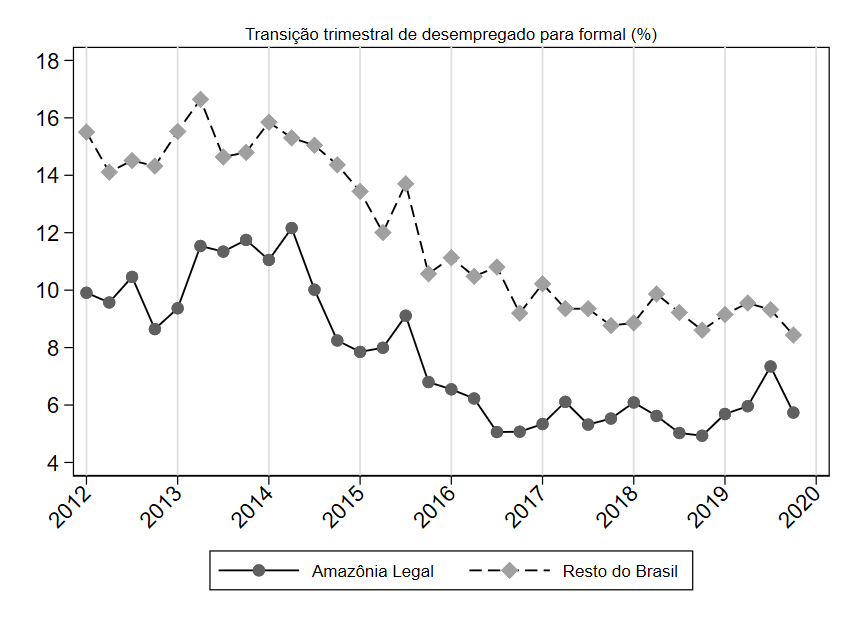
\includegraphics[width=1\linewidth]{../../analysis/output/transicao_ocupacao/_transicao_ocupacao_sh_desempregado_sh_formal.png}
  \caption{}
  \label{fig:_transicao_ocupacao_sh_desempregado_sh_formal}
\end{figure}
\end{frame}

\begin{frame}[label=_transicao_ocupacao_sh_desempregado_sh_informal]{}
\textit{\hyperlink{_transicao_ocupacao}{\beamerbutton{Voltar}}}
\begin{figure}
  \centering
  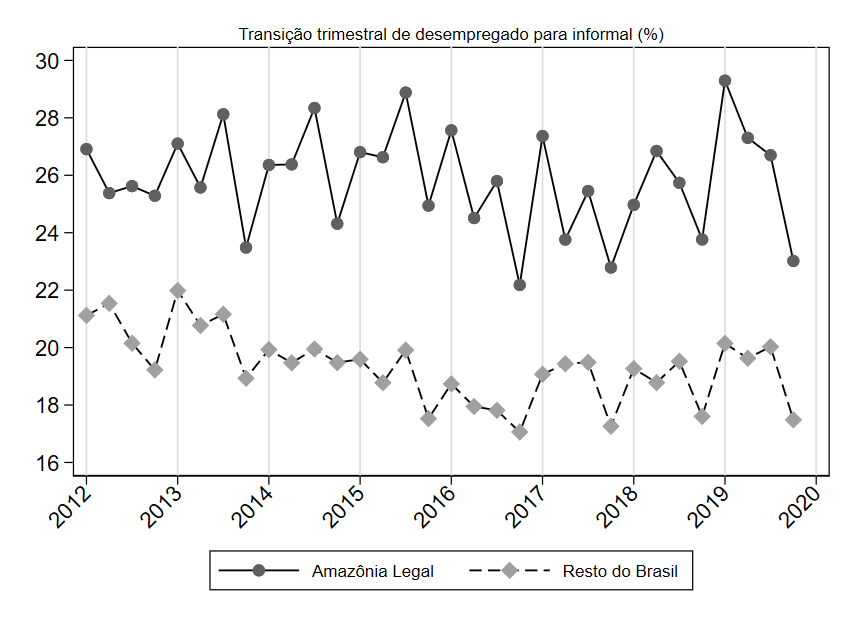
\includegraphics[width=1.0\linewidth]{../../analysis/output/transicao_ocupacao/_transicao_ocupacao_sh_desempregado_sh_informal.png}
  \caption{}
  \label{fig:_transicao_ocupacao_sh_desempregado_sh_informal}
\end{figure}
\end{frame}

\begin{frame}[label=_transicao_ocupacao_sh_desempregado_sh_inativa]{}
\textit{\hyperlink{_transicao_ocupacao}{\beamerbutton{Voltar}}}
\begin{figure}
  \centering
  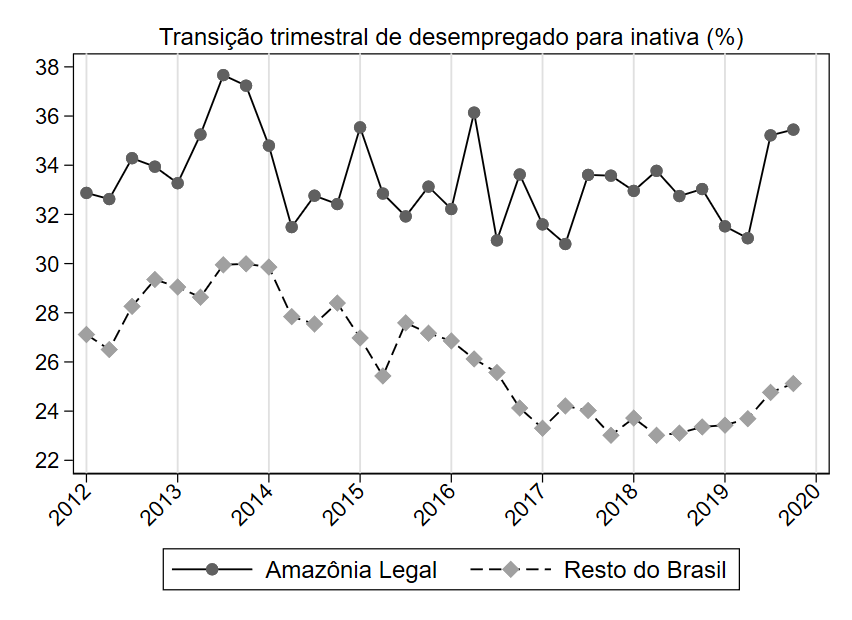
\includegraphics[width=1.0\linewidth]{../../analysis/output/transicao_ocupacao/_transicao_ocupacao_sh_desempregado_sh_inativa.png}
  \caption{}
  \label{fig:_transicao_ocupacao_sh_desempregado_sh_inativa}
\end{figure}
\end{frame}

\begin{frame}[label=_transicao_ocupacao_sh_formal_sh_desempregado]{}
\textit{\hyperlink{_transicao_ocupacao}{\beamerbutton{Voltar}}}
\begin{figure}
  \centering
  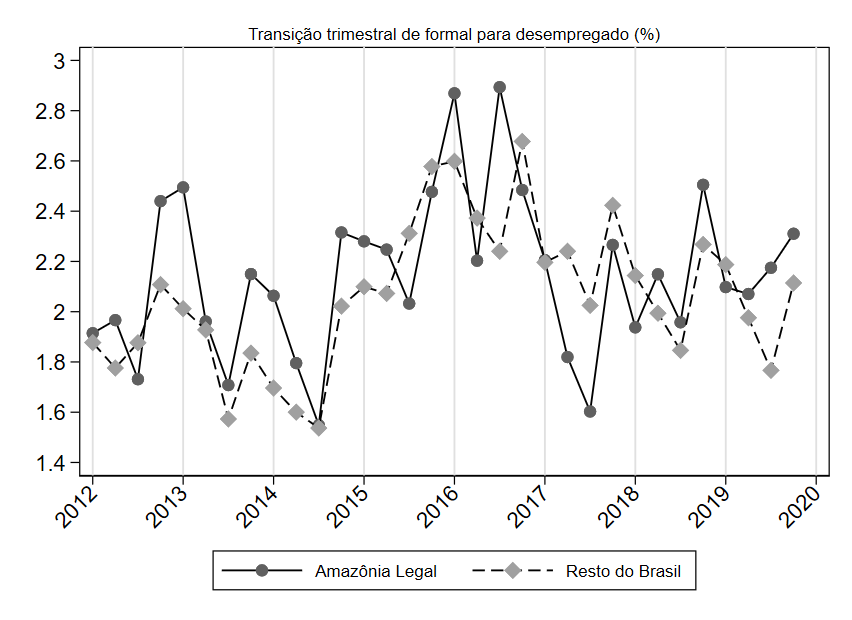
\includegraphics[width=1.0\linewidth]{../../analysis/output/transicao_ocupacao/_transicao_ocupacao_sh_formal_sh_desempregado.png}
  \caption{}
  \label{fig:_transicao_ocupacao_sh_formal_sh_desempregado}
\end{figure}
\end{frame}


\begin{frame}[label=_transicao_ocupacao_sh_formal_sh_inativa]{}
\textit{\hyperlink{_transicao_ocupacao}{\beamerbutton{Voltar}}}
\begin{figure}
  \centering
  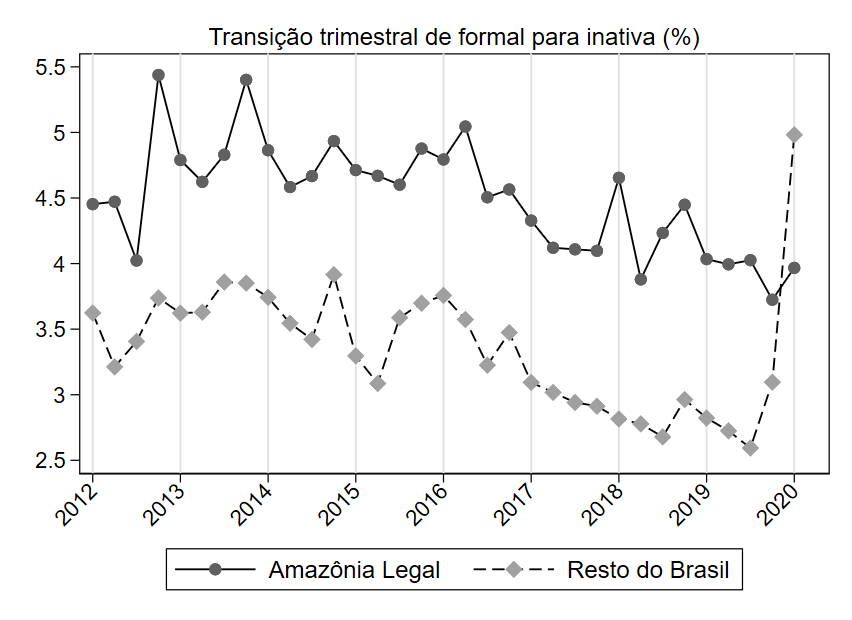
\includegraphics[width=1.0\linewidth]{../../analysis/output/transicao_ocupacao/_transicao_ocupacao_sh_formal_sh_inativa.png}
  \caption{}
  \label{fig:_transicao_ocupacao_sh_formal_sh_inativa}
\end{figure}
\end{frame}

\begin{frame}[label=_transicao_ocupacao_sh_formal_sh_informal]{}
\textit{\hyperlink{_transicao_ocupacao}{\beamerbutton{Voltar}}}
\begin{figure}
  \centering
  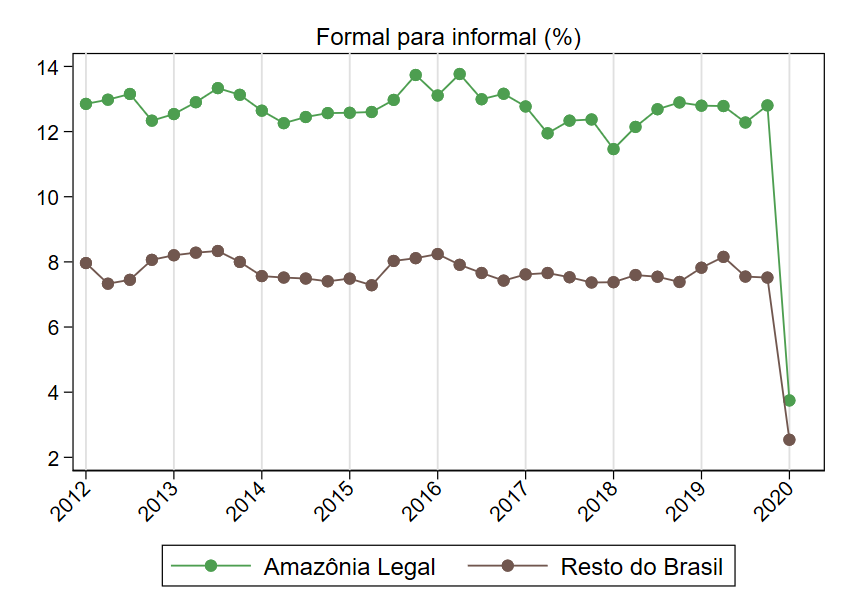
\includegraphics[width=1.0\linewidth]{../../analysis/output/transicao_ocupacao/_transicao_ocupacao_sh_formal_sh_informal.png}
  \caption{}
  \label{fig:_transicao_ocupacao_sh_formal_sh_informal}
\end{figure}
\end{frame}

\begin{frame}[label=_transicao_ocupacao_sh_informal_sh_desempregado]{}
\textit{\hyperlink{_transicao_ocupacao}{\beamerbutton{Voltar}}}
\begin{figure}
  \centering
  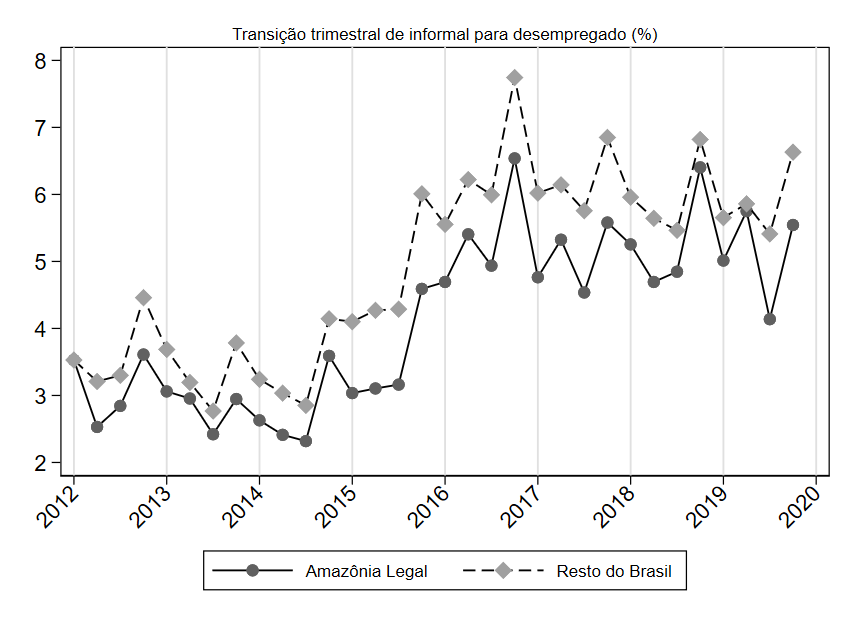
\includegraphics[width=1.0\linewidth]{../../analysis/output/transicao_ocupacao/_transicao_ocupacao_sh_informal_sh_desempregado.png}
  \caption{}
  \label{fig:_transicao_ocupacao_sh_informal_sh_desempregado}
\end{figure}
\end{frame}



\begin{frame}[label=_transicao_ocupacao_sh_informal_sh_formal]{}
\textit{\hyperlink{_transicao_ocupacao}{\beamerbutton{Voltar}}}
\begin{figure}
  \centering
  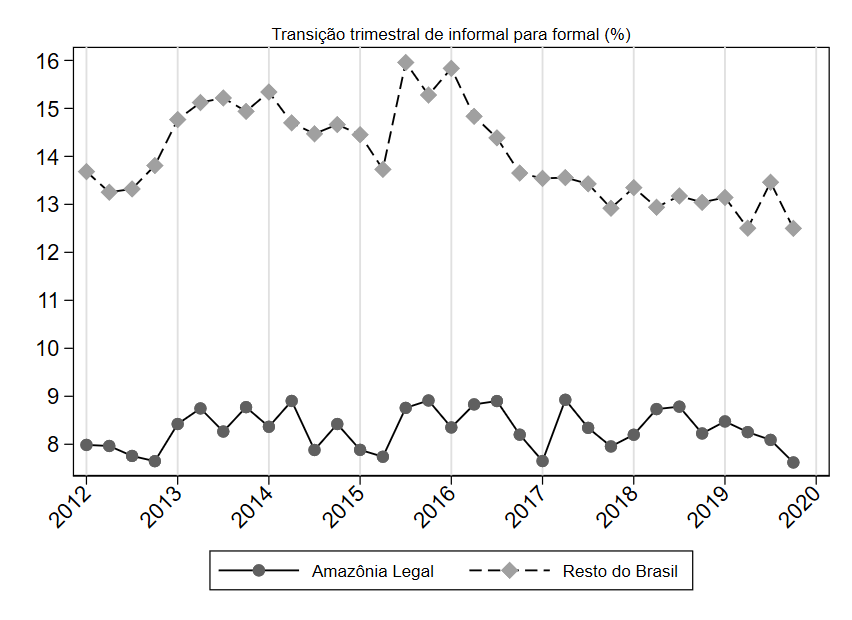
\includegraphics[width=1.0\linewidth]{../../analysis/output/transicao_ocupacao/_transicao_ocupacao_sh_informal_sh_formal.png}
  \caption{}
  \label{fig:_transicao_ocupacao_sh_informal_sh_formal}
\end{figure}
\end{frame}

\begin{frame}[label=_transicao_ocupacao_sh_informal_sh_inativa]{}
\textit{\hyperlink{_transicao_ocupacao}{\beamerbutton{Voltar}}}
\begin{figure}
  \centering
  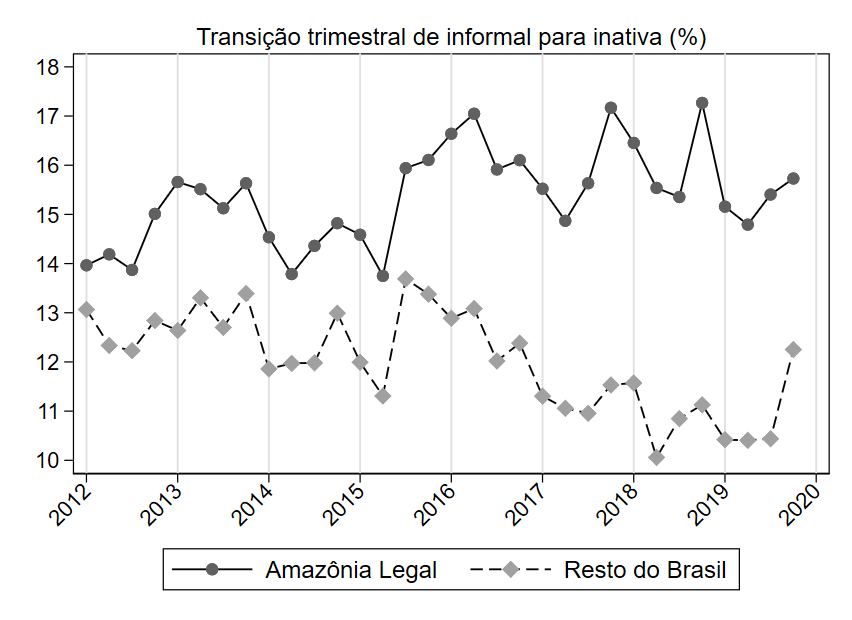
\includegraphics[width=1.0\linewidth]{../../analysis/output/transicao_ocupacao/_transicao_ocupacao_sh_informal_sh_inativa.png}
  \caption{}
  \label{fig:_transicao_ocupacao_sh_informal_sh_inativa}
\end{figure}
\end{frame}


\section{Composição Demográfica}

\begin{frame}[label=_composicao_demografica]{Composição Demográfica}
{\footnotesize Fonte de dados: Dados da PNAD Contínua Anual (2012-2019)}



\begin{itemize}
\item{
	\hyperlink{_composicao_demografica_raca}{\beamerbutton{Raça}}
	}   
		
\item{
	\hyperlink{_composicao_demografica_genero}{\beamerbutton{Gênero}}
	}  
	
\item{
	\hyperlink{_composicao_demografica_faixa_etaria}{\beamerbutton{Faixa etária}}
	}  
	
\item{
	\hyperlink{_composicao_demografica_educacao}{\beamerbutton{Educação}} 
	}  
	
\item{
	\hyperlink{_composicao_demografica_setor}{\beamerbutton{Setor ocupacional}}
	}  
	
\item{
	\hyperlink{_composicao_demografica_regiao_metro}{\beamerbutton{Regiões metropolitanas}} 
	}
\item{
	\hyperlink{_composicao_demografica_rural_urbano}{\beamerbutton{Zona rural vs. zona urbana}} 
	} 	  

\end{itemize}
\begin{small}
\textit{Retornar ao índice principal: \hyperlink{indice_principal}{\beamerbutton{AQUI}} }
\end{small}
\end{frame}


\begin{frame}[label=_composicao_demografica_raca]{Composição Demográfica: Raça}
{\footnotesize Fonte de dados: Dados da PNAD Contínua Trimestral (2012-2020)}
\begin{itemize}
\item{Taxa de ocupação: \hyperlink{_composicao_demografica_raca_taxa_de_ocupacao}{\beamerbutton{clique aqui}}}
\item{Taxa de informalidade: \hyperlink{_composicao_demografica_raca_taxa_de_informalidade}{\beamerbutton{clique aqui}}}
\item{Taxa de desemprego: \hyperlink{_composicao_demografica_raca_taxa_de_desemprego}{\beamerbutton{clique aqui}}}
\item{Taxa de participação: \hyperlink{_composicao_demografica_raca_taxa_de_participacao}{\beamerbutton{clique aqui}}}
\item{Proporção de servidores públicos e militares: \hyperlink{_composicao_demografica_raca_prop_militar}{\beamerbutton{clique aqui}}}
\item{Proporção de empregados sem carteira: \hyperlink{_composicao_demografica_raca_prop_empregadoSC}{\beamerbutton{clique aqui}}}
\item{Proporção de empregados com carteira: \hyperlink{_composicao_demografica_raca_prop_empregadoCC}{\beamerbutton{clique aqui}}}
\item{Proporção de empregadores \hyperlink{_composicao_demografica_raca_prop_empregador}{\beamerbutton{clique aqui}}}
\item{Proporção de conta própria: \hyperlink{_composicao_demografica_raca_prop_cpropria}{\beamerbutton{clique aqui}}}
\item{Proporção de conta própria que contribui: \hyperlink{_composicao_demografica_raca_prop_cpropriaC}{\beamerbutton{clique aqui}}}
\item{Proporção de conta própria que não contribui: \hyperlink{_composicao_demografica_raca_prop_cpropriaNc}{\beamerbutton{clique aqui}}}
\end{itemize}

\begin{small}
\textit{Retornar ao índice principal da composição demográfica: \hyperlink{_composicao_demografica}{\beamerbutton{AQUI}} }
\end{small}

\end{frame}

\begin{frame}[label=_composicao_demografica_raca_taxa_de_ocupacao]{}
\textit{\hyperlink{_composicao_demografica_raca}{\beamerbutton{Voltar}}}
\begin{figure}
  \centering
  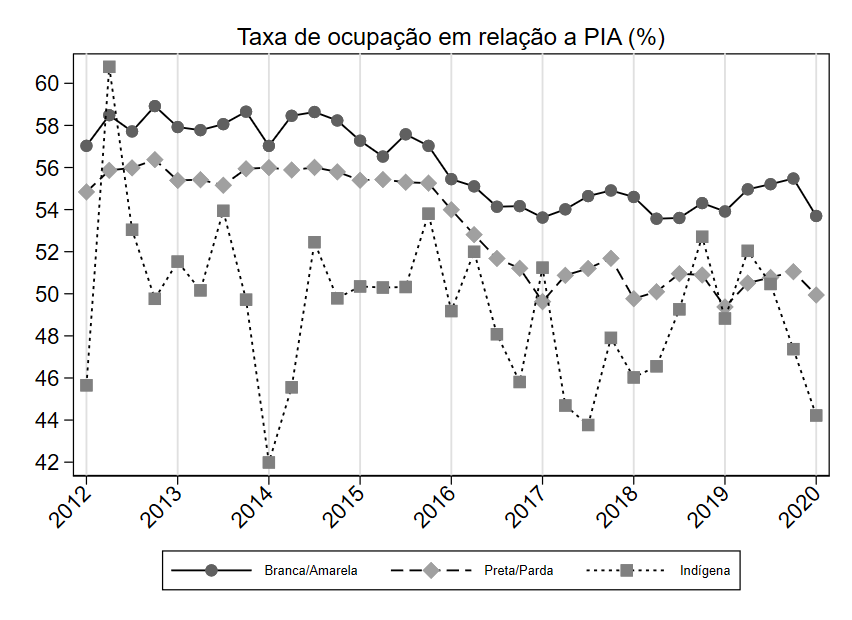
\includegraphics[width=1\linewidth]{../../analysis/output/composicao_demografica/raca/_composicao_demografica_raca_taxa_de_ocupacao.png}
  \caption{}
  \label{fig:_composicao_demografica_raca_taxa_de_ocupacao}
\end{figure}
\end{frame}

\begin{frame}[label=_composicao_demografica_raca_taxa_de_informalidade]{}
\textit{\hyperlink{_composicao_demografica_raca}{\beamerbutton{Voltar}}}
\begin{figure}
  \centering
  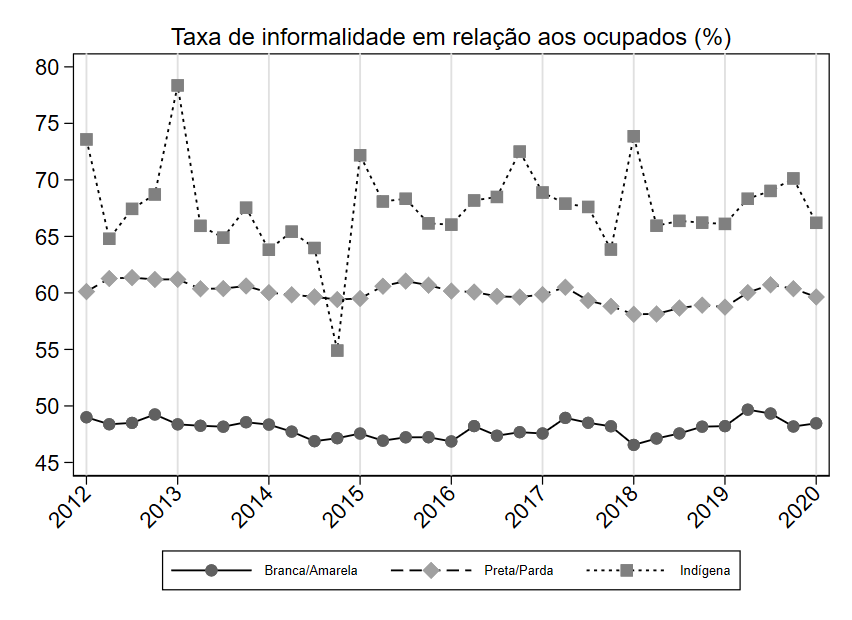
\includegraphics[width=1.0\linewidth]{../../analysis/output/composicao_demografica/raca/_composicao_demografica_raca_taxa_de_informalidade.png}
  \caption{}
  \label{fig:_composicao_demografica_raca_taxa_de_informalidade}
\end{figure}
\end{frame}

\begin{frame}[label=_composicao_demografica_raca_taxa_de_desemprego]{}
\textit{\hyperlink{_composicao_demografica_raca}{\beamerbutton{Voltar}}}
\begin{figure}
  \centering
  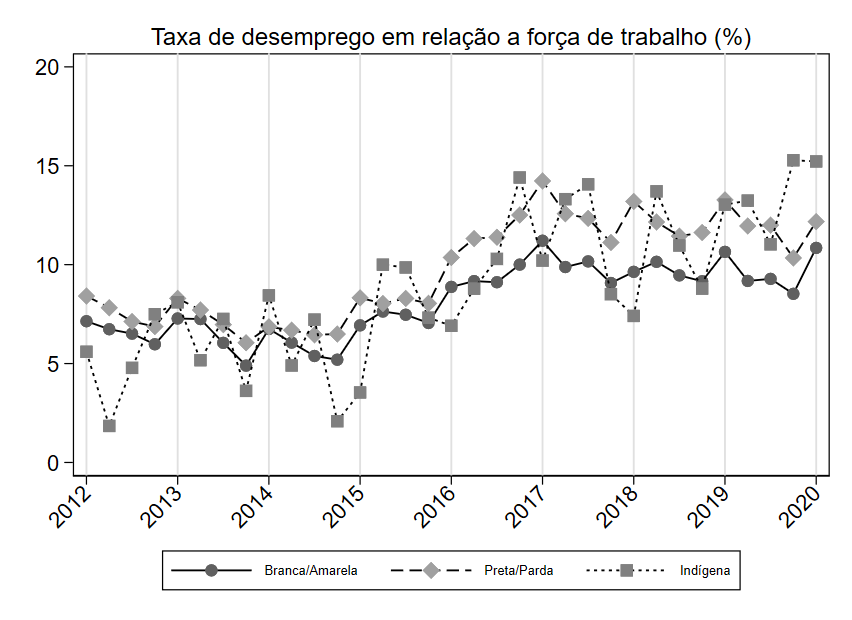
\includegraphics[width=1.0\linewidth]{../../analysis/output/composicao_demografica/raca/_composicao_demografica_raca_taxa_de_desemprego.png}
  \caption{}
  \label{fig:_composicao_demografica_raca_taxa_de_desemprego}
\end{figure}
\end{frame}

\begin{frame}[label=_composicao_demografica_raca_taxa_de_participacao]{}
\textit{\hyperlink{_composicao_demografica_raca}{\beamerbutton{Voltar}}}
\begin{figure}
  \centering
  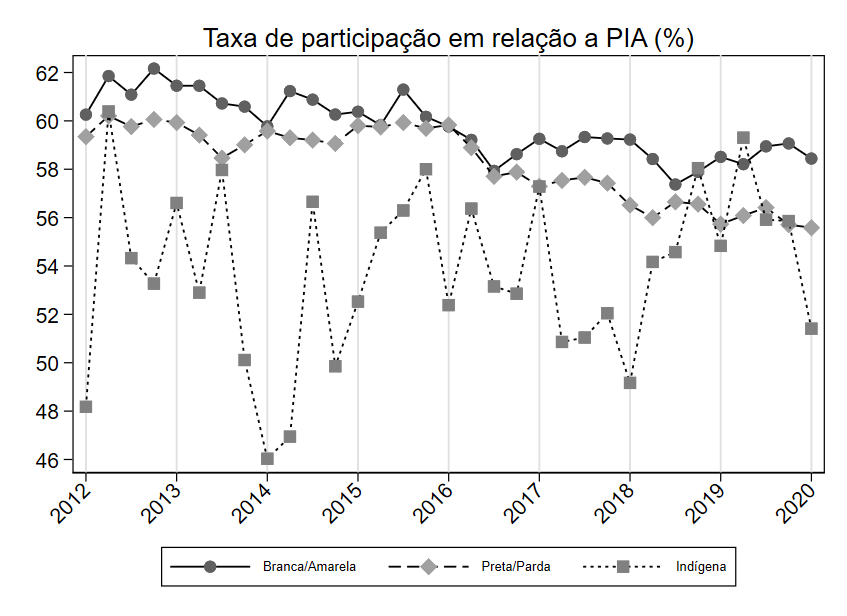
\includegraphics[width=1.0\linewidth]{../../analysis/output/composicao_demografica/raca/_composicao_demografica_raca_taxa_de_participacao.png}
  \caption{}
  \label{fig:_composicao_demografica_raca_taxa_de_participacao}
\end{figure}
\end{frame}

\begin{frame}[label=_composicao_demografica_raca_prop_militar]{}
\textit{\hyperlink{_composicao_demografica_raca}{\beamerbutton{Voltar}}}
\begin{figure}
  \centering
  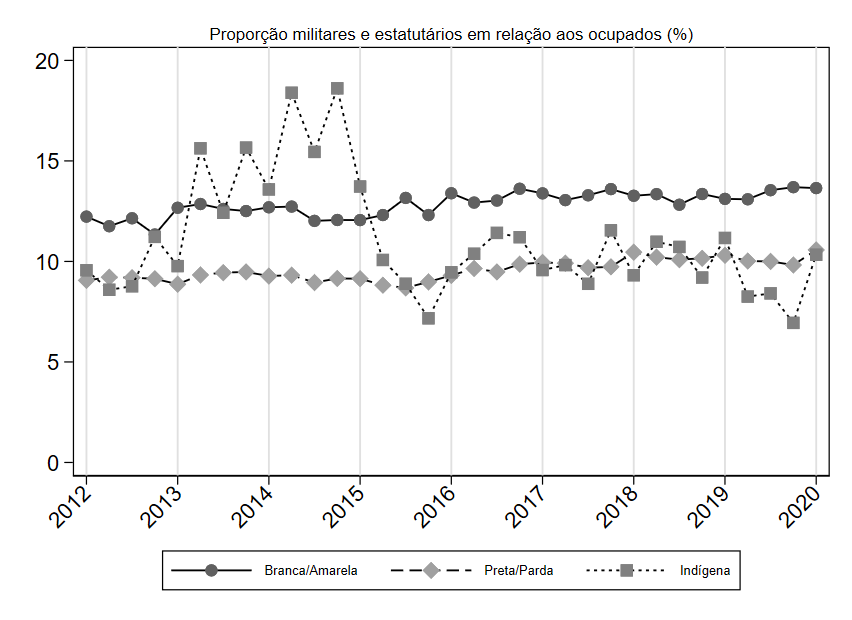
\includegraphics[width=1.0\linewidth]{../../analysis/output/composicao_demografica/raca/_composicao_demografica_raca_prop_militar.png}
  \caption{}
  \label{fig:_composicao_demografica_raca_prop_militar}
\end{figure}
\end{frame}


\begin{frame}[label=_composicao_demografica_raca_prop_empregadoSC]{}
\textit{\hyperlink{_composicao_demografica_raca}{\beamerbutton{Voltar}}}
\begin{figure}
  \centering
  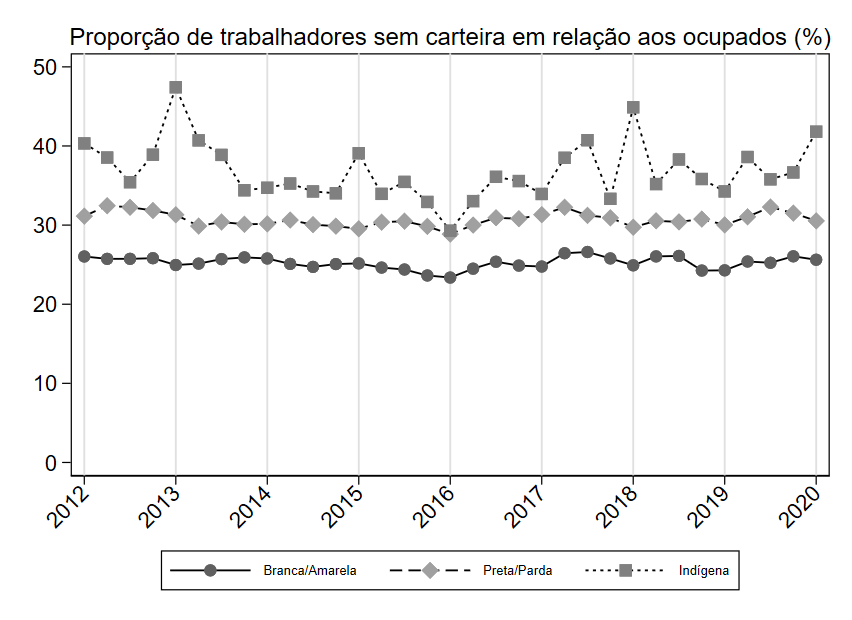
\includegraphics[width=1.0\linewidth]{../../analysis/output/composicao_demografica/raca/_composicao_demografica_raca_prop_empregadoSC.png}
  \caption{}
  \label{fig:_composicao_demografica_raca_prop_empregadoSC}
\end{figure}
\end{frame}

\begin{frame}[label=_composicao_demografica_raca_prop_empregadoCC]{}
\textit{\hyperlink{_composicao_demografica_raca}{\beamerbutton{Voltar}}}
\begin{figure}
  \centering
  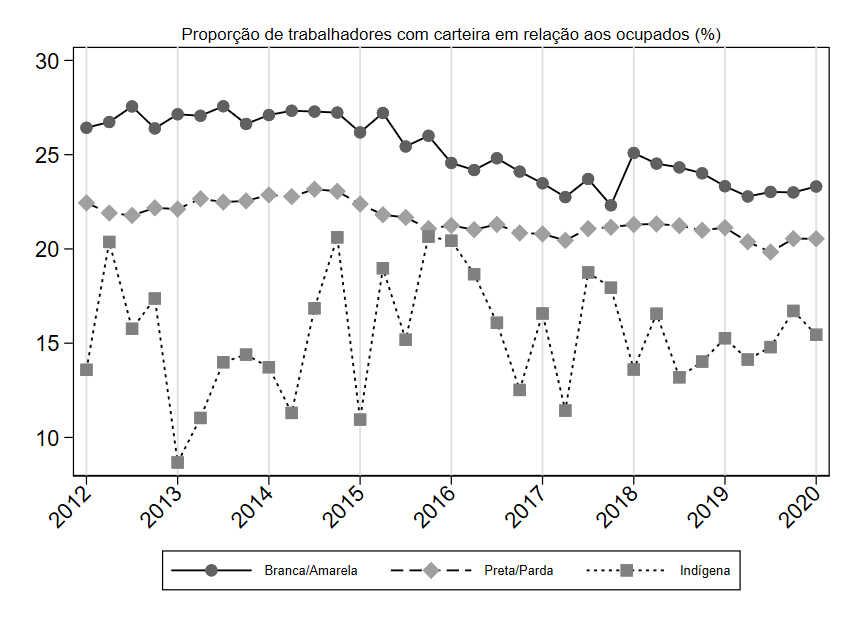
\includegraphics[width=1.0\linewidth]{../../analysis/output/composicao_demografica/raca/_composicao_demografica_raca_prop_empregadoCC.png}
  \caption{}
  \label{fig:_composicao_demografica_raca_prop_empregadoCC}
\end{figure}
\end{frame}

\begin{frame}[label=_composicao_demografica_raca_prop_empregador]{}
\textit{\hyperlink{_composicao_demografica_raca}{\beamerbutton{Voltar}}}
\begin{figure}
  \centering
  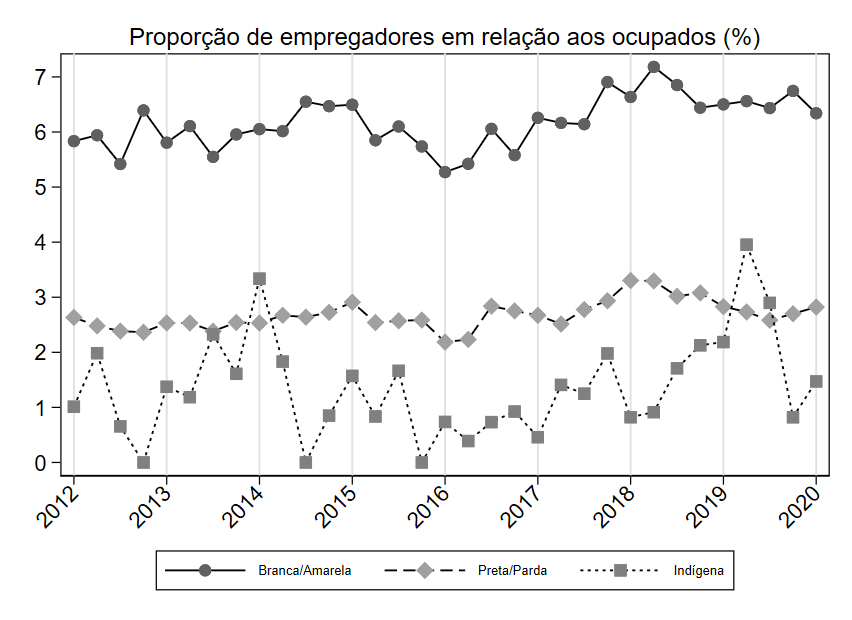
\includegraphics[width=1.0\linewidth]{../../analysis/output/composicao_demografica/raca/_composicao_demografica_raca_prop_empregador.png}
  \caption{}
  \label{fig:_composicao_demografica_raca_prop_empregador}
\end{figure}
\end{frame}



\begin{frame}[label=_composicao_demografica_raca_prop_cpropria]{}
\textit{\hyperlink{_composicao_demografica_raca}{\beamerbutton{Voltar}}}
\begin{figure}
  \centering
  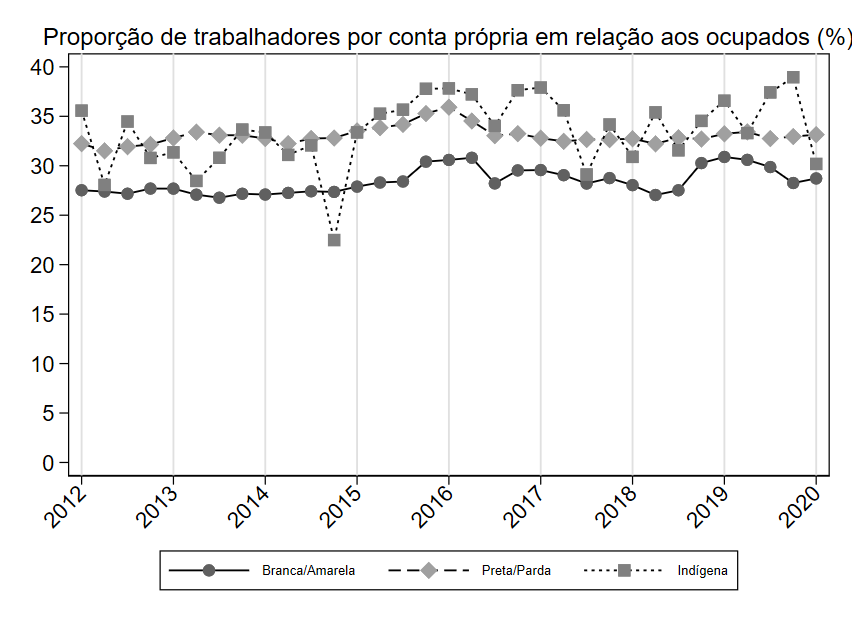
\includegraphics[width=1.0\linewidth]{../../analysis/output/composicao_demografica/raca/_composicao_demografica_raca_prop_cpropria.png}
  \caption{}
  \label{fig:_composicao_demografica_raca_prop_cpropria}
\end{figure}
\end{frame}

\begin{frame}[label=_composicao_demografica_raca_prop_cpropriaC]{}
\textit{\hyperlink{_composicao_demografica_raca}{\beamerbutton{Voltar}}}
\begin{figure}
  \centering
  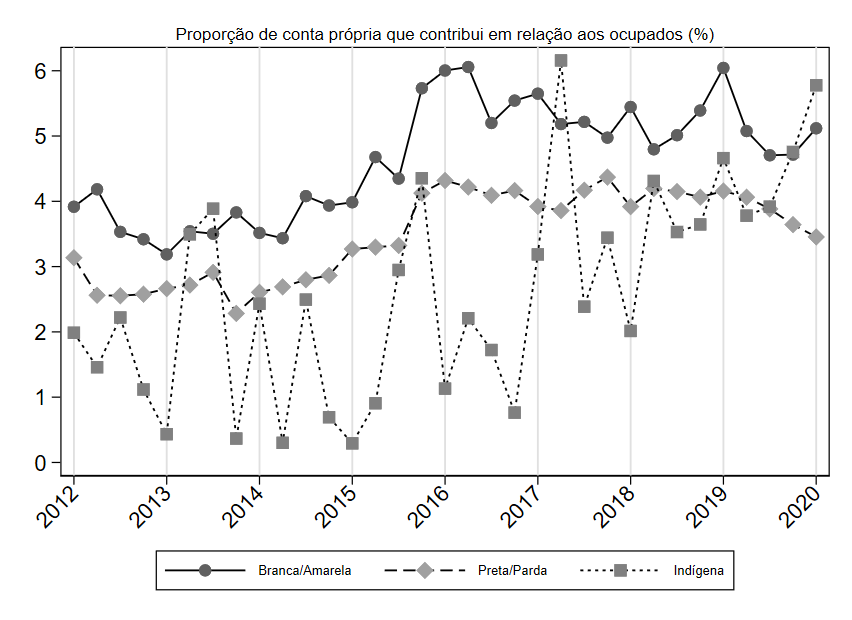
\includegraphics[width=1.0\linewidth]{../../analysis/output/composicao_demografica/raca/_composicao_demografica_raca_prop_cpropriaC.png}
  \caption{}
  \label{fig:_composicao_demografica_raca_prop_cpropriaC}
\end{figure}
\end{frame}

\begin{frame}[label=_composicao_demografica_raca_prop_cpropriaNc]{}
\textit{\hyperlink{_composicao_demografica_raca}{\beamerbutton{Voltar}}}
\begin{figure}
  \centering
  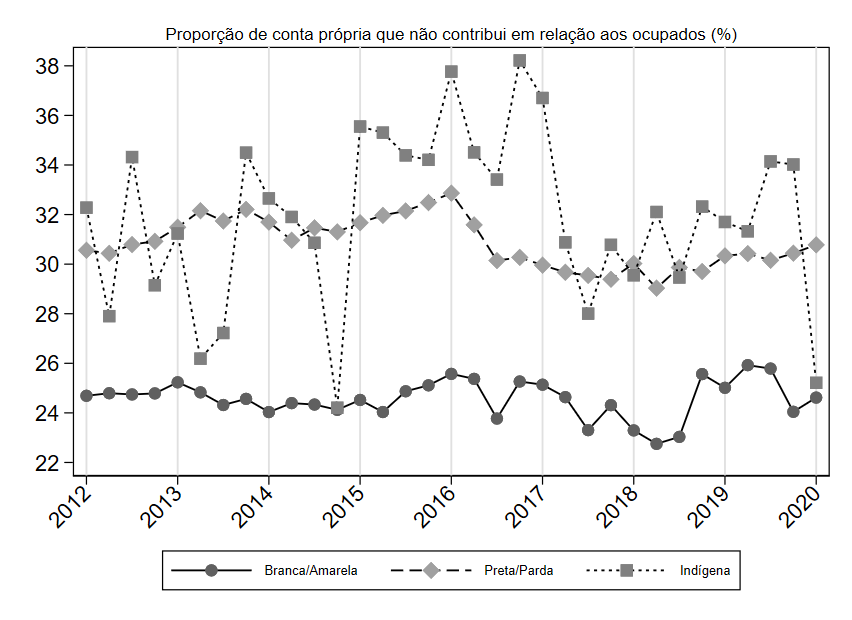
\includegraphics[width=1.0\linewidth]{../../analysis/output/composicao_demografica/raca/_composicao_demografica_raca_prop_cpropriaNc.png}
  \caption{}
  \label{fig:_composicao_demografica_raca_prop_cpropriaNc}
\end{figure}
\end{frame}
\begin{frame}[label=_composicao_demografica_genero]{Composição Demográfica: Gênero}
{\footnotesize Fonte de dados: Dados da PNAD Contínua Trimestral (2012-2020)}
\begin{itemize}
\item{Taxa de ocupação: \hyperlink{_composicao_demografica_genero_taxa_de_ocupacao}{\beamerbutton{clique aqui}}}
\item{Taxa de informalidade: \hyperlink{_composicao_demografica_genero_taxa_de_informalidade}{\beamerbutton{clique aqui}}}
\item{Taxa de desemprego: \hyperlink{_composicao_demografica_genero_taxa_de_desemprego}{\beamerbutton{clique aqui}}}
\item{Taxa de participação: \hyperlink{_composicao_demografica_genero_taxa_de_participacao}{\beamerbutton{clique aqui}}}
\item{Proporção de militares e estatutários: \hyperlink{_composicao_demografica_genero_prop_militar}{\beamerbutton{clique aqui}}}
\item{Proporção de empregados sem carteira: \hyperlink{_composicao_demografica_genero_prop_empregadoSC}{\beamerbutton{clique aqui}}}
\item{Proporção de empregados com carteira: \hyperlink{_composicao_demografica_genero_prop_empregadoCC}{\beamerbutton{clique aqui}}}
\item{Proporção de empregadores \hyperlink{_composicao_demografica_genero_prop_empregador}{\beamerbutton{clique aqui}}}
\item{Proporção de conta própria: \hyperlink{_composicao_demografica_genero_prop_cpropria}{\beamerbutton{clique aqui}}}
\item{Proporção de conta própria que contribui: \hyperlink{_composicao_demografica_genero_prop_cpropriaC}{\beamerbutton{clique aqui}}}
\item{Proporção de conta própria que não contribui: \hyperlink{_composicao_demografica_genero_prop_cpropriaNc}{\beamerbutton{clique aqui}}}
\end{itemize}

\begin{small}
\textit{Retornar ao índice principal da composição demográfica: \hyperlink{_composicao_demografica}{\beamerbutton{AQUI}} }
\end{small}

\end{frame}

\begin{frame}[label=_composicao_demografica_genero_taxa_de_ocupacao]{}
\textit{\hyperlink{_composicao_demografica_genero}{\beamerbutton{Voltar}}}
\begin{figure}
  \centering
  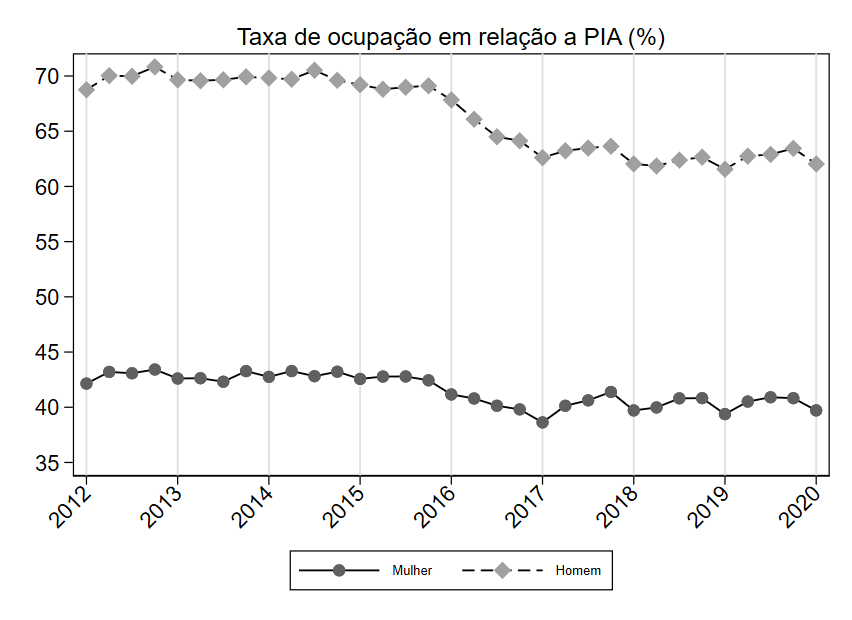
\includegraphics[width=1\linewidth]{../../analysis/output/composicao_demografica/genero/_composicao_demografica_genero_taxa_de_ocupacao.png}
  \caption{}
  \label{fig:_composicao_demografica_genero_taxa_de_ocupacao}
\end{figure}
\end{frame}

\begin{frame}[label=_composicao_demografica_genero_taxa_de_informalidade]{}
\textit{\hyperlink{_composicao_demografica_genero}{\beamerbutton{Voltar}}}
\begin{figure}
  \centering
  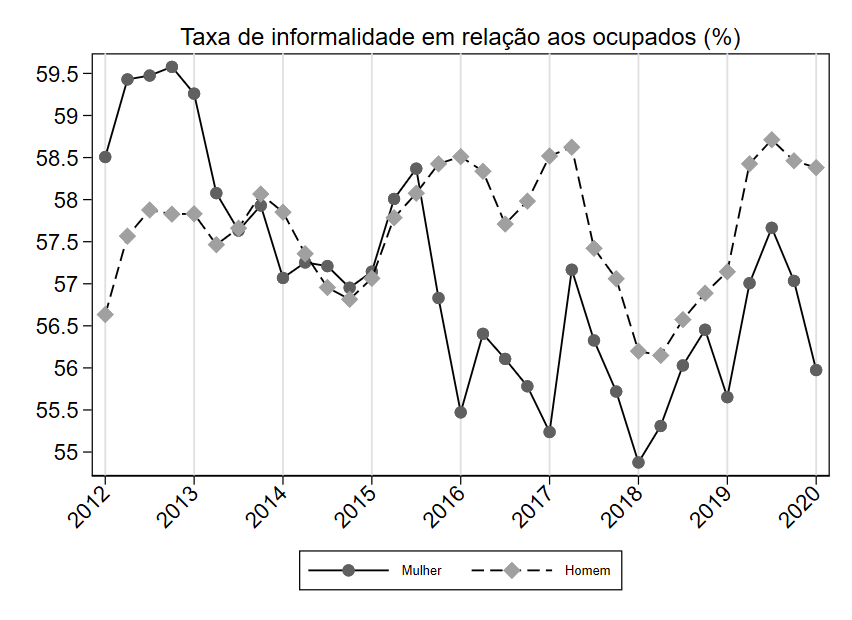
\includegraphics[width=1.0\linewidth]{../../analysis/output/composicao_demografica/genero/_composicao_demografica_genero_taxa_de_informalidade.png}
  \caption{}
  \label{fig:_composicao_demografica_genero_taxa_de_informalidade}
\end{figure}
\end{frame}

\begin{frame}[label=_composicao_demografica_genero_taxa_de_desemprego]{}
\textit{\hyperlink{_composicao_demografica_genero}{\beamerbutton{Voltar}}}
\begin{figure}
  \centering
  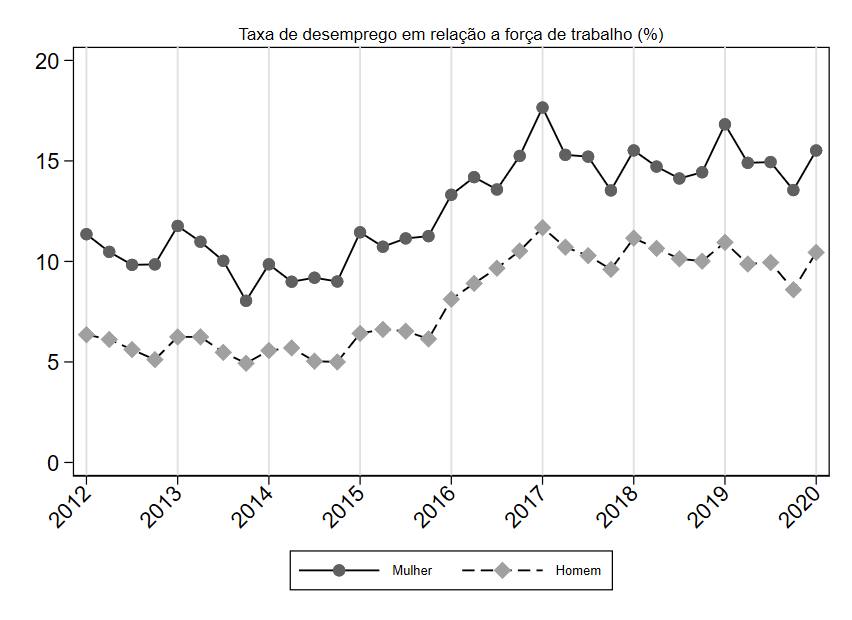
\includegraphics[width=1.0\linewidth]{../../analysis/output/composicao_demografica/genero/_composicao_demografica_genero_taxa_de_desemprego.png}
  \caption{}
  \label{fig:_composicao_demografica_genero_taxa_de_desemprego}
\end{figure}
\end{frame}

\begin{frame}[label=_composicao_demografica_genero_taxa_de_participacao]{}
\textit{\hyperlink{_composicao_demografica_genero}{\beamerbutton{Voltar}}}
\begin{figure}
  \centering
  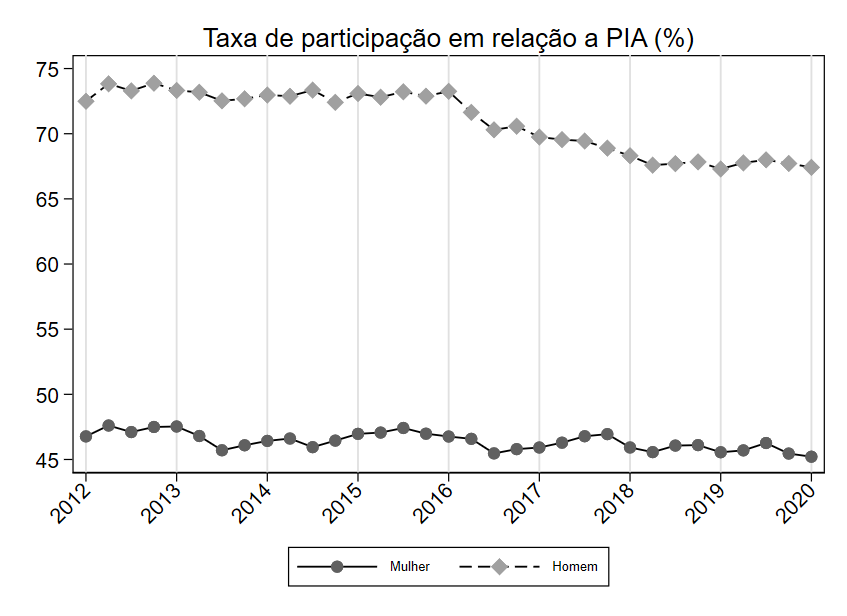
\includegraphics[width=1.0\linewidth]{../../analysis/output/composicao_demografica/genero/_composicao_demografica_genero_taxa_de_participacao.png}
  \caption{}
  \label{fig:_composicao_demografica_genero_taxa_de_participacao}
\end{figure}
\end{frame}

\begin{frame}[label=_composicao_demografica_genero_prop_militar]{}
\textit{\hyperlink{_composicao_demografica_genero}{\beamerbutton{Voltar}}}
\begin{figure}
  \centering
  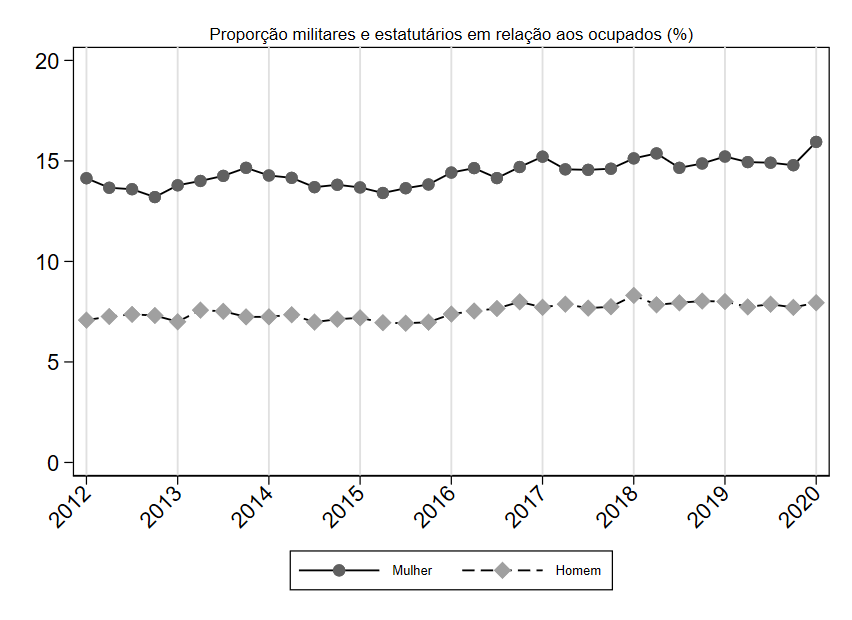
\includegraphics[width=1.0\linewidth]{../../analysis/output/composicao_demografica/genero/_composicao_demografica_genero_prop_militar.png}
  \caption{}
  \label{fig:_composicao_demografica_genero_prop_militar}
\end{figure}
\end{frame}


\begin{frame}[label=_composicao_demografica_genero_prop_empregadoSC]{}
\textit{\hyperlink{_composicao_demografica_genero}{\beamerbutton{Voltar}}}
\begin{figure}
  \centering
  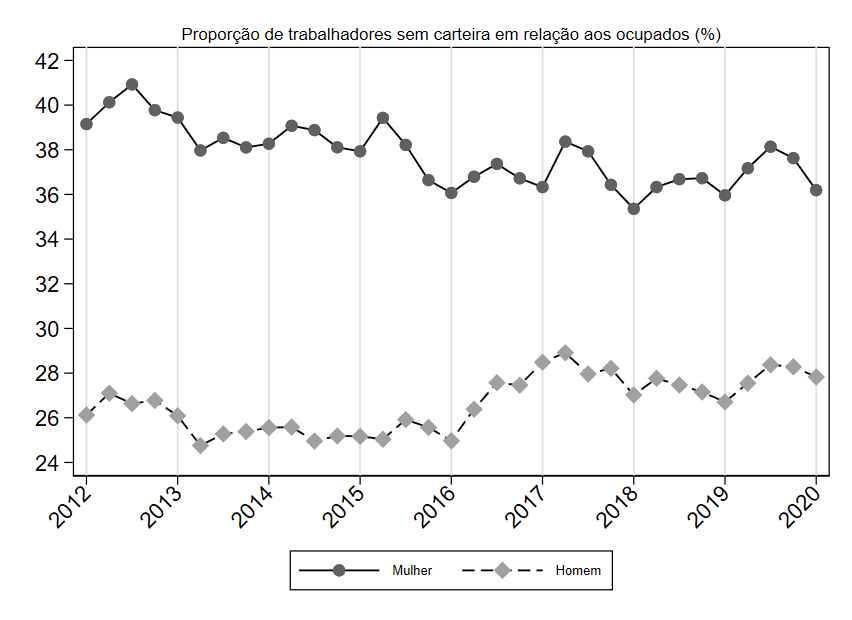
\includegraphics[width=1.0\linewidth]{../../analysis/output/composicao_demografica/genero/_composicao_demografica_genero_prop_empregadoSC.png}
  \caption{}
  \label{fig:_composicao_demografica_genero_prop_empregadoSC}
\end{figure}
\end{frame}

\begin{frame}[label=_composicao_demografica_genero_prop_empregadoCC]{}
\textit{\hyperlink{_composicao_demografica_genero}{\beamerbutton{Voltar}}}
\begin{figure}
  \centering
  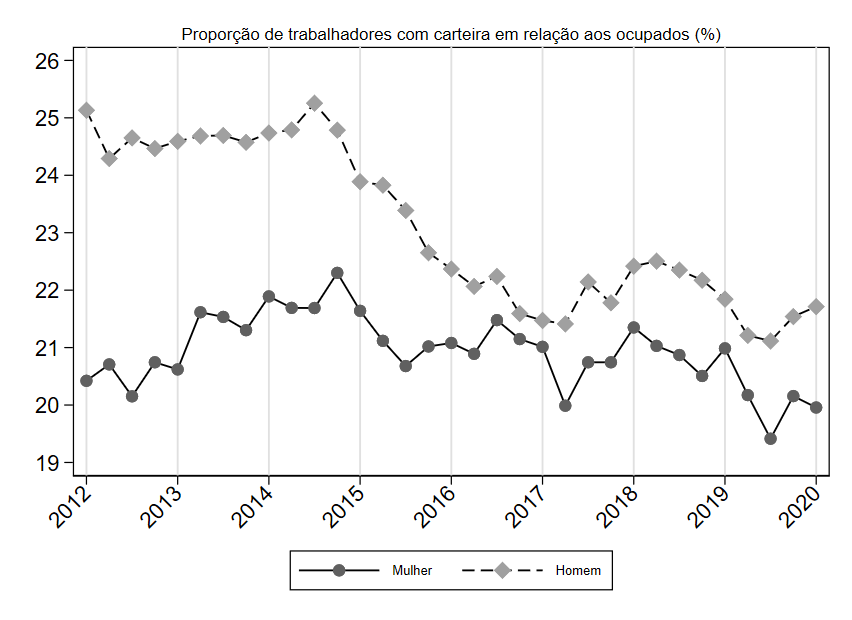
\includegraphics[width=1.0\linewidth]{../../analysis/output/composicao_demografica/genero/_composicao_demografica_genero_prop_empregadoCC.png}
  \caption{}
  \label{fig:_composicao_demografica_genero_prop_empregadoCC}
\end{figure}
\end{frame}

\begin{frame}[label=_composicao_demografica_genero_prop_empregador]{}
\textit{\hyperlink{_composicao_demografica_genero}{\beamerbutton{Voltar}}}
\begin{figure}
  \centering
  \includegraphics[width=1.0\linewidth]{../../analysis/output/composicao_demografica/genero/_composicao_demografica_genero_prop_empregador.png}
  \caption{}
  \label{fig:_composicao_demografica_genero_prop_empregador}
\end{figure}
\end{frame}



\begin{frame}[label=_composicao_demografica_genero_prop_cpropria]{}
\textit{\hyperlink{_composicao_demografica_genero}{\beamerbutton{Voltar}}}
\begin{figure}
  \centering
  \includegraphics[width=1.0\linewidth]{../../analysis/output/composicao_demografica/genero/_composicao_demografica_genero_prop_cpropria.png}
  \caption{}
  \label{fig:_composicao_demografica_genero_prop_cpropria}
\end{figure}
\end{frame}

\begin{frame}[label=_composicao_demografica_genero_prop_cpropriaC]{}
\textit{\hyperlink{_composicao_demografica_genero}{\beamerbutton{Voltar}}}
\begin{figure}
  \centering
  \includegraphics[width=1.0\linewidth]{../../analysis/output/composicao_demografica/genero/_composicao_demografica_genero_prop_cpropriaC.png}
  \caption{}
  \label{fig:_composicao_demografica_genero_prop_cpropriaC}
\end{figure}
\end{frame}

\begin{frame}[label=_composicao_demografica_genero_prop_cpropriaNc]{}
\textit{\hyperlink{_composicao_demografica_genero}{\beamerbutton{Voltar}}}
\begin{figure}
  \centering
  \includegraphics[width=1.0\linewidth]{../../analysis/output/composicao_demografica/genero/_composicao_demografica_genero_prop_cpropriaNc.png}
  \caption{}
  \label{fig:_composicao_demografica_genero_prop_cpropriaNc}
\end{figure}
\end{frame}
\begin{frame}[label=_composicao_demografica_faixa_etaria]{Composição Demográfica: Faixa Etária}
{\footnotesize Fonte de dados: Dados da PNAD Contínua Trimestral (2012-2020)}
\begin{itemize}
\item{Taxa de ocupação: \hyperlink{_composicao_demografica_faixa_etaria_taxa_de_ocupacao}{\beamerbutton{clique aqui}}}
\item{Taxa de informalidade: \hyperlink{_composicao_demografica_faixa_etaria_taxa_de_informalidade}{\beamerbutton{clique aqui}}}
\item{Taxa de desemprego: \hyperlink{_composicao_demografica_faixa_etaria_taxa_de_desemprego}{\beamerbutton{clique aqui}}}
\item{Proporção de militares e estatutários: \hyperlink{_composicao_demografica_faixa_etaria_prop_militar}{\beamerbutton{clique aqui}}}
\item{Proporção de empregados sem carteira: \hyperlink{_composicao_demografica_faixa_etaria_prop_empregadoSC}{\beamerbutton{clique aqui}}}
\item{Proporção de empregados com carteira: \hyperlink{_composicao_demografica_faixa_etaria_prop_empregadoCC}{\beamerbutton{clique aqui}}}
\item{Proporção de empregadores \hyperlink{_composicao_demografica_faixa_etaria_prop_empregador}{\beamerbutton{clique aqui}}}
\item{Proporção de conta própria: \hyperlink{_composicao_demografica_faixa_etaria_prop_cpropria}{\beamerbutton{clique aqui}}}
\item{Proporção de conta própria que contribui: \hyperlink{_composicao_demografica_faixa_etaria_prop_cpropriaC}{\beamerbutton{clique aqui}}}
\item{Proporção de conta própria que não contribui: \hyperlink{_composicao_demografica_faixa_etaria_prop_cpropriaNc}{\beamerbutton{clique aqui}}}
\end{itemize}

\begin{small}
\textit{Retornar ao índice principal da composição demográfica: \hyperlink{_composicao_demografica}{\beamerbutton{AQUI}} }
\end{small}

\end{frame}

\begin{frame}[label=_composicao_demografica_faixa_etaria_taxa_de_ocupacao]{}
\textit{\hyperlink{_composicao_demografica_faixa_etaria}{\beamerbutton{Voltar}}}
\begin{figure}
  \centering
  \includegraphics[width=1\linewidth]{../../analysis/output/composicao_demografica/faixa_etaria/_composicao_demografica_faixa_etaria_taxa_de_ocupacao.png}
  \caption{}
  \label{fig:_composicao_demografica_faixa_etaria_taxa_de_ocupacao}
\end{figure}
\end{frame}

\begin{frame}[label=_composicao_demografica_faixa_etaria_taxa_de_informalidade]{}
\textit{\hyperlink{_composicao_demografica_faixa_etaria}{\beamerbutton{Voltar}}}
\begin{figure}
  \centering
  \includegraphics[width=1.0\linewidth]{../../analysis/output/composicao_demografica/faixa_etaria/_composicao_demografica_faixa_etaria_taxa_de_informalidade.png}
  \caption{}
  \label{fig:_composicao_demografica_faixa_etaria_taxa_de_informalidade}
\end{figure}
\end{frame}

\begin{frame}[label=_composicao_demografica_faixa_etaria_taxa_de_desemprego]{}
\textit{\hyperlink{_composicao_demografica_faixa_etaria}{\beamerbutton{Voltar}}}
\begin{figure}
  \centering
  \includegraphics[width=1.0\linewidth]{../../analysis/output/composicao_demografica/faixa_etaria/_composicao_demografica_faixa_etaria_taxa_de_desemprego.png}
  \caption{}
  \label{fig:_composicao_demografica_faixa_etaria_taxa_de_desemprego}
\end{figure}
\end{frame}

\begin{frame}[label=_composicao_demografica_faixa_etaria_prop_militar]{}
\textit{\hyperlink{_composicao_demografica_faixa_etaria}{\beamerbutton{Voltar}}}
\begin{figure}
  \centering
  \includegraphics[width=1.0\linewidth]{../../analysis/output/composicao_demografica/faixa_etaria/_composicao_demografica_faixa_etaria_prop_militar.png}
  \caption{}
  \label{fig:_composicao_demografica_faixa_etaria_prop_militar}
\end{figure}
\end{frame}


\begin{frame}[label=_composicao_demografica_faixa_etaria_prop_empregadoSC]{}
\textit{\hyperlink{_composicao_demografica_faixa_etaria}{\beamerbutton{Voltar}}}
\begin{figure}
  \centering
  \includegraphics[width=1.0\linewidth]{../../analysis/output/composicao_demografica/faixa_etaria/_composicao_demografica_faixa_etaria_prop_empregadoSC.png}
  \caption{}
  \label{fig:_composicao_demografica_faixa_etaria_prop_empregadoSC}
\end{figure}
\end{frame}

\begin{frame}[label=_composicao_demografica_faixa_etaria_prop_empregadoCC]{}
\textit{\hyperlink{_composicao_demografica_faixa_etaria}{\beamerbutton{Voltar}}}
\begin{figure}
  \centering
  \includegraphics[width=1.0\linewidth]{../../analysis/output/composicao_demografica/faixa_etaria/_composicao_demografica_faixa_etaria_prop_empregadoCC.png}
  \caption{}
  \label{fig:_composicao_demografica_faixa_etaria_prop_empregadoCC}
\end{figure}
\end{frame}

\begin{frame}[label=_composicao_demografica_faixa_etaria_prop_empregador]{}
\textit{\hyperlink{_composicao_demografica_faixa_etaria}{\beamerbutton{Voltar}}}
\begin{figure}
  \centering
  \includegraphics[width=1.0\linewidth]{../../analysis/output/composicao_demografica/faixa_etaria/_composicao_demografica_faixa_etaria_prop_empregador.png}
  \caption{}
  \label{fig:_composicao_demografica_faixa_etaria_prop_empregador}
\end{figure}
\end{frame}



\begin{frame}[label=_composicao_demografica_faixa_etaria_prop_cpropria]{}
\textit{\hyperlink{_composicao_demografica_faixa_etaria}{\beamerbutton{Voltar}}}
\begin{figure}
  \centering
  \includegraphics[width=1.0\linewidth]{../../analysis/output/composicao_demografica/faixa_etaria/_composicao_demografica_faixa_etaria_prop_cpropria.png}
  \caption{}
  \label{fig:_composicao_demografica_faixa_etaria_prop_cpropria}
\end{figure}
\end{frame}

\begin{frame}[label=_composicao_demografica_faixa_etaria_prop_cpropriaC]{}
\textit{\hyperlink{_composicao_demografica_faixa_etaria}{\beamerbutton{Voltar}}}
\begin{figure}
  \centering
  \includegraphics[width=1.0\linewidth]{../../analysis/output/composicao_demografica/faixa_etaria/_composicao_demografica_faixa_etaria_prop_cpropriaC.png}
  \caption{}
  \label{fig:_composicao_demografica_faixa_etaria_prop_cpropriaC}
\end{figure}
\end{frame}

\begin{frame}[label=_composicao_demografica_faixa_etaria_prop_cpropriaNc]{}
\textit{\hyperlink{_composicao_demografica_faixa_etaria}{\beamerbutton{Voltar}}}
\begin{figure}
  \centering
  \includegraphics[width=1.0\linewidth]{../../analysis/output/composicao_demografica/faixa_etaria/_composicao_demografica_faixa_etaria_prop_cpropriaNc.png}
  \caption{}
  \label{fig:_composicao_demografica_faixa_etaria_prop_cpropriaNc}
\end{figure}
\end{frame}
\begin{frame}[label=_composicao_demografica_educacao]{Composição Demográfica: Educação}
{\footnotesize Fonte de dados: Dados da PNAD Contínua Trimestral (2012-2020)}
\begin{itemize}
\item{Taxa de ocupação: \hyperlink{_composicao_demografica_educacao_taxa_de_ocupacao}{\beamerbutton{clique aqui}}}
\item{Taxa de informalidade: \hyperlink{_composicao_demografica_educacao_taxa_de_informalidade}{\beamerbutton{clique aqui}}}
\item{Taxa de desemprego: \hyperlink{_composicao_demografica_educacao_taxa_de_desemprego}{\beamerbutton{clique aqui}}}
\item{Taxa de participação: \hyperlink{_composicao_demografica_educacao_taxa_de_participacao}{\beamerbutton{clique aqui}}}
\item{Proporção de servidores públicos e militares: \hyperlink{_composicao_demografica_educacao_prop_militar}{\beamerbutton{clique aqui}}}
\item{Proporção de empregados sem carteira: \hyperlink{_composicao_demografica_educacao_prop_empregadoSC}{\beamerbutton{clique aqui}}}
\item{Proporção de empregados com carteira: \hyperlink{_composicao_demografica_educacao_prop_empregadoCC}{\beamerbutton{clique aqui}}}
\item{Proporção de empregadores \hyperlink{_composicao_demografica_educacao_prop_empregador}{\beamerbutton{clique aqui}}}
\item{Proporção de conta própria: \hyperlink{_composicao_demografica_educacao_prop_cpropria}{\beamerbutton{clique aqui}}}
\item{Proporção de conta própria que contribui: \hyperlink{_composicao_demografica_educacao_prop_cpropriaC}{\beamerbutton{clique aqui}}}
\item{Proporção de conta própria que não contribui: \hyperlink{_composicao_demografica_educacao_prop_cpropriaNc}{\beamerbutton{clique aqui}}}
\end{itemize}

\begin{small}
\textit{Retornar ao índice principal da composição demográfica: \hyperlink{_composicao_demografica}{\beamerbutton{AQUI}} }
\end{small}

\end{frame}

\begin{frame}[label=_composicao_demografica_educacao_taxa_de_ocupacao]{}
\textit{\hyperlink{_composicao_demografica_educacao}{\beamerbutton{Voltar}}}
\begin{figure}
  \centering
  \includegraphics[width=1\linewidth]{../../analysis/output/composicao_demografica/educacao/_composicao_demografica_educacao_taxa_de_ocupacao.png}
  \caption{}
  \label{fig:_composicao_demografica_educacao_taxa_de_ocupacao}
\end{figure}
\end{frame}

\begin{frame}[label=_composicao_demografica_educacao_taxa_de_informalidade]{}
\textit{\hyperlink{_composicao_demografica_educacao}{\beamerbutton{Voltar}}}
\begin{figure}
  \centering
  \includegraphics[width=1.0\linewidth]{../../analysis/output/composicao_demografica/educacao/_composicao_demografica_educacao_taxa_de_informalidade.png}
  \caption{}
  \label{fig:_composicao_demografica_educacao_taxa_de_informalidade}
\end{figure}
\end{frame}

\begin{frame}[label=_composicao_demografica_educacao_taxa_de_desemprego]{}
\textit{\hyperlink{_composicao_demografica_educacao}{\beamerbutton{Voltar}}}
\begin{figure}
  \centering
  \includegraphics[width=1.0\linewidth]{../../analysis/output/composicao_demografica/educacao/_composicao_demografica_educacao_taxa_de_desemprego.png}
  \caption{}
  \label{fig:_composicao_demografica_educacao_taxa_de_desemprego}
\end{figure}
\end{frame}

\begin{frame}[label=_composicao_demografica_educacao_taxa_de_participacao]{}
\textit{\hyperlink{_composicao_demografica_educacao}{\beamerbutton{Voltar}}}
\begin{figure}
  \centering
  \includegraphics[width=1.0\linewidth]{../../analysis/output/composicao_demografica/educacao/_composicao_demografica_educacao_taxa_de_participacao.png}
  \caption{}
  \label{fig:_composicao_demografica_educacao_taxa_de_participacao}
\end{figure}
\end{frame}

\begin{frame}[label=_composicao_demografica_educacao_prop_militar]{}
\textit{\hyperlink{_composicao_demografica_educacao}{\beamerbutton{Voltar}}}
\begin{figure}
  \centering
  \includegraphics[width=1.0\linewidth]{../../analysis/output/composicao_demografica/educacao/_composicao_demografica_educacao_prop_militar.png}
  \caption{}
  \label{fig:_composicao_demografica_educacao_prop_militar}
\end{figure}
\end{frame}


\begin{frame}[label=_composicao_demografica_educacao_prop_empregadoSC]{}
\textit{\hyperlink{_composicao_demografica_educacao}{\beamerbutton{Voltar}}}
\begin{figure}
  \centering
  \includegraphics[width=1.0\linewidth]{../../analysis/output/composicao_demografica/educacao/_composicao_demografica_educacao_prop_empregadoSC.png}
  \caption{}
  \label{fig:_composicao_demografica_educacao_prop_empregadoSC}
\end{figure}
\end{frame}

\begin{frame}[label=_composicao_demografica_educacao_prop_empregadoCC]{}
\textit{\hyperlink{_composicao_demografica_educacao}{\beamerbutton{Voltar}}}
\begin{figure}
  \centering
  \includegraphics[width=1.0\linewidth]{../../analysis/output/composicao_demografica/educacao/_composicao_demografica_educacao_prop_empregadoCC.png}
  \caption{}
  \label{fig:_composicao_demografica_educacao_prop_empregadoCC}
\end{figure}
\end{frame}

\begin{frame}[label=_composicao_demografica_educacao_prop_empregador]{}
\textit{\hyperlink{_composicao_demografica_educacao}{\beamerbutton{Voltar}}}
\begin{figure}
  \centering
  \includegraphics[width=1.0\linewidth]{../../analysis/output/composicao_demografica/educacao/_composicao_demografica_educacao_prop_empregador.png}
  \caption{}
  \label{fig:_composicao_demografica_educacao_prop_empregador}
\end{figure}
\end{frame}



\begin{frame}[label=_composicao_demografica_educacao_prop_cpropria]{}
\textit{\hyperlink{_composicao_demografica_educacao}{\beamerbutton{Voltar}}}
\begin{figure}
  \centering
  \includegraphics[width=1.0\linewidth]{../../analysis/output/composicao_demografica/educacao/_composicao_demografica_educacao_prop_cpropria.png}
  \caption{}
  \label{fig:_composicao_demografica_educacao_prop_cpropria}
\end{figure}
\end{frame}

\begin{frame}[label=_composicao_demografica_educacao_prop_cpropriaC]{}
\textit{\hyperlink{_composicao_demografica_educacao}{\beamerbutton{Voltar}}}
\begin{figure}
  \centering
  \includegraphics[width=1.0\linewidth]{../../analysis/output/composicao_demografica/educacao/_composicao_demografica_educacao_prop_cpropriaC.png}
  \caption{}
  \label{fig:_composicao_demografica_educacao_prop_cpropriaC}
\end{figure}
\end{frame}

\begin{frame}[label=_composicao_demografica_educacao_prop_cpropriaNc]{}
\textit{\hyperlink{_composicao_demografica_educacao}{\beamerbutton{Voltar}}}
\begin{figure}
  \centering
  \includegraphics[width=1.0\linewidth]{../../analysis/output/composicao_demografica/educacao/_composicao_demografica_educacao_prop_cpropriaNc.png}
  \caption{}
  \label{fig:_composicao_demografica_educacao_prop_cpropriaNc}
\end{figure}
\end{frame}
\begin{frame}[label=_composicao_demografica_setor]{Composição Demográfica: Setor Ocupacional}
{\footnotesize Fonte de dados: Dados da PNAD Contínua Trimestral (2012-2020)}
\begin{itemize}
\item{Taxa de informalidade: \hyperlink{_composicao_demografica_setor_taxa_de_informalidade}{\beamerbutton{clique aqui}}}
\item{Proporção deservidores públicos e militares: \hyperlink{_composicao_demografica_setor_prop_militar}{\beamerbutton{clique aqui}}}
\item{Proporção de empregados sem carteira: \hyperlink{_composicao_demografica_setor_prop_empregadoSC}{\beamerbutton{clique aqui}}}
\item{Proporção de empregados com carteira: \hyperlink{_composicao_demografica_setor_prop_empregadoCC}{\beamerbutton{clique aqui}}}
\item{Proporção de empregadores \hyperlink{_composicao_demografica_setor_prop_empregador}{\beamerbutton{clique aqui}}}
\item{Proporção de conta própria: \hyperlink{_composicao_demografica_setor_prop_cpropria}{\beamerbutton{clique aqui}}}
\item{Proporção de conta própria que contribui: \hyperlink{_composicao_demografica_setor_prop_cpropriaC}{\beamerbutton{clique aqui}}}
\item{Proporção de conta própria que não contribui: \hyperlink{_composicao_demografica_setor_prop_cpropriaNc}{\beamerbutton{clique aqui}}}
\end{itemize}

\begin{small}
\textit{Retornar ao índice principal da composição demográfica: \hyperlink{_composicao_demografica}{\beamerbutton{AQUI}} }
\end{small}

\end{frame}


\begin{frame}[label=_composicao_demografica_setor_taxa_de_informalidade]{}
\textit{\hyperlink{_composicao_demografica_setor}{\beamerbutton{Voltar}}}
\begin{figure}
  \centering
  \includegraphics[width=1.0\linewidth]{../../analysis/output/composicao_demografica/setor/_composicao_demografica_setor_taxa_de_informalidade.png}
  \caption{}
  \label{fig:_composicao_demografica_setor_taxa_de_informalidade}
\end{figure}
\end{frame}


\begin{frame}[label=_composicao_demografica_setor_prop_militar]{}
\textit{\hyperlink{_composicao_demografica_setor}{\beamerbutton{Voltar}}}
\begin{figure}
  \centering
  \includegraphics[width=1.0\linewidth]{../../analysis/output/composicao_demografica/setor/_composicao_demografica_setor_prop_militar.png}
  \caption{}
  \label{fig:_composicao_demografica_setor_prop_militar}
\end{figure}
\end{frame}


\begin{frame}[label=_composicao_demografica_setor_prop_empregadoSC]{}
\textit{\hyperlink{_composicao_demografica_setor}{\beamerbutton{Voltar}}}
\begin{figure}
  \centering
  \includegraphics[width=1.0\linewidth]{../../analysis/output/composicao_demografica/setor/_composicao_demografica_setor_prop_empregadoSC.png}
  \caption{}
  \label{fig:_composicao_demografica_setor_prop_empregadoSC}
\end{figure}
\end{frame}

\begin{frame}[label=_composicao_demografica_setor_prop_empregadoCC]{}
\textit{\hyperlink{_composicao_demografica_setor}{\beamerbutton{Voltar}}}
\begin{figure}
  \centering
  \includegraphics[width=1.0\linewidth]{../../analysis/output/composicao_demografica/setor/_composicao_demografica_setor_prop_empregadoCC.png}
  \caption{}
  \label{fig:_composicao_demografica_setor_prop_empregadoCC}
\end{figure}
\end{frame}

\begin{frame}[label=_composicao_demografica_setor_prop_empregador]{}
\textit{\hyperlink{_composicao_demografica_setor}{\beamerbutton{Voltar}}}
\begin{figure}
  \centering
  \includegraphics[width=1.0\linewidth]{../../analysis/output/composicao_demografica/setor/_composicao_demografica_setor_prop_empregador.png}
  \caption{}
  \label{fig:_composicao_demografica_setor_prop_empregador}
\end{figure}
\end{frame}



\begin{frame}[label=_composicao_demografica_setor_prop_cpropria]{}
\textit{\hyperlink{_composicao_demografica_setor}{\beamerbutton{Voltar}}}
\begin{figure}
  \centering
  \includegraphics[width=1.0\linewidth]{../../analysis/output/composicao_demografica/setor/_composicao_demografica_setor_prop_cpropria.png}
  \caption{}
  \label{fig:_composicao_demografica_setor_prop_cpropria}
\end{figure}
\end{frame}

\begin{frame}[label=_composicao_demografica_setor_prop_cpropriaC]{}
\textit{\hyperlink{_composicao_demografica_setor}{\beamerbutton{Voltar}}}
\begin{figure}
  \centering
  \includegraphics[width=1.0\linewidth]{../../analysis/output/composicao_demografica/setor/_composicao_demografica_setor_prop_cpropriaC.png}
  \caption{}
  \label{fig:_composicao_demografica_setor_prop_cpropriaC}
\end{figure}
\end{frame}

\begin{frame}[label=_composicao_demografica_setor_prop_cpropriaNc]{}
\textit{\hyperlink{_composicao_demografica_setor}{\beamerbutton{Voltar}}}
\begin{figure}
  \centering
  \includegraphics[width=1.0\linewidth]{../../analysis/output/composicao_demografica/setor/_composicao_demografica_setor_prop_cpropriaNc.png}
  \caption{}
  \label{fig:_composicao_demografica_setor_prop_cpropriaNc}
\end{figure}
\end{frame}
\begin{frame}[label=_composicao_demografica_regiao_metro]{Composição Demográfica: Regiões metropolitanas}
{\footnotesize Fonte de dados: Dados da PNAD Contínua Trimestral (2012-2020)}
\begin{itemize}
\item{Taxa de ocupação: \hyperlink{_composicao_demografica_regiao_metro_taxa_de_ocupacao}{\beamerbutton{clique aqui}}}
\item{Taxa de informalidade: \hyperlink{_composicao_demografica_regiao_metro_taxa_de_informalidade}{\beamerbutton{clique aqui}}}
\item{Taxa de desemprego: \hyperlink{_composicao_demografica_regiao_metro_taxa_de_desemprego}{\beamerbutton{clique aqui}}}
\item{Taxa de participação: \hyperlink{_composicao_demografica_regiao_metro_taxa_de_participacao}{\beamerbutton{clique aqui}}}
\item{Proporção de servidores públicos e militares: \hyperlink{_composicao_demografica_regiao_metro_prop_militar}{\beamerbutton{clique aqui}}}
\item{Proporção de empregados sem carteira: \hyperlink{_composicao_demografica_regiao_metro_prop_empregadoSC}{\beamerbutton{clique aqui}}}
\item{Proporção de empregados com carteira: \hyperlink{_composicao_demografica_regiao_metro_prop_empregadoCC}{\beamerbutton{clique aqui}}}
\item{Proporção de empregadores \hyperlink{_composicao_demografica_regiao_metro_prop_empregador}{\beamerbutton{clique aqui}}}
\item{Proporção de conta própria: \hyperlink{_composicao_demografica_regiao_metro_prop_cpropria}{\beamerbutton{clique aqui}}}
\item{Proporção de conta própria que contribui: \hyperlink{_composicao_demografica_regiao_metro_prop_cpropriaC}{\beamerbutton{clique aqui}}}
\item{Proporção de conta própria que não contribui: \hyperlink{_composicao_demografica_regiao_metro_prop_cpropriaNc}{\beamerbutton{clique aqui}}}
\end{itemize}

\begin{small}
\textit{Retornar ao índice principal da composição demográfica: \hyperlink{_composicao_demografica}{\beamerbutton{AQUI}} }
\end{small}

\end{frame}

\begin{frame}[label=_composicao_demografica_regiao_metro_taxa_de_ocupacao]{}
\textit{\hyperlink{_composicao_demografica_regiao_metro}{\beamerbutton{Voltar}}}
\begin{figure}
  \centering
  \includegraphics[width=1\linewidth]{../../analysis/output/composicao_demografica/area_geografica/_composicao_demografica_regiao_metro_taxa_de_ocupacao.png}
  \caption{}
  \label{fig:_composicao_demografica_regiao_metro_taxa_de_ocupacao}
\end{figure}
\end{frame}

\begin{frame}[label=_composicao_demografica_regiao_metro_taxa_de_informalidade]{}
\textit{\hyperlink{_composicao_demografica_regiao_metro}{\beamerbutton{Voltar}}}
\begin{figure}
  \centering
  \includegraphics[width=1.0\linewidth]{../../analysis/output/composicao_demografica/area_geografica/_composicao_demografica_regiao_metro_taxa_de_informalidade.png}
  \caption{}
  \label{fig:_composicao_demografica_regiao_metro_taxa_de_informalidade}
\end{figure}
\end{frame}

\begin{frame}[label=_composicao_demografica_regiao_metro_taxa_de_desemprego]{}
\textit{\hyperlink{_composicao_demografica_regiao_metro}{\beamerbutton{Voltar}}}
\begin{figure}
  \centering
  \includegraphics[width=1.0\linewidth]{../../analysis/output/composicao_demografica/area_geografica/_composicao_demografica_regiao_metro_taxa_de_desemprego.png}
  \caption{}
  \label{fig:_composicao_demografica_regiao_metro_taxa_de_desemprego}
\end{figure}
\end{frame}

\begin{frame}[label=_composicao_demografica_regiao_metro_taxa_de_participacao]{}
\textit{\hyperlink{_composicao_demografica_regiao_metro}{\beamerbutton{Voltar}}}
\begin{figure}
  \centering
  \includegraphics[width=1.0\linewidth]{../../analysis/output/composicao_demografica/area_geografica/_composicao_demografica_regiao_metro_taxa_de_participacao.png}
  \caption{}
  \label{fig:_composicao_demografica_regiao_metro_taxa_de_participacao}
\end{figure}
\end{frame}

\begin{frame}[label=_composicao_demografica_regiao_metro_prop_militar]{}
\textit{\hyperlink{_composicao_demografica_regiao_metro}{\beamerbutton{Voltar}}}
\begin{figure}
  \centering
  \includegraphics[width=1.0\linewidth]{../../analysis/output/composicao_demografica/area_geografica/_composicao_demografica_regiao_metro_prop_militar.png}
  \caption{}
  \label{fig:_composicao_demografica_regiao_metro_prop_militar}
\end{figure}
\end{frame}


\begin{frame}[label=_composicao_demografica_regiao_metro_prop_empregadoSC]{}
\textit{\hyperlink{_composicao_demografica_regiao_metro}{\beamerbutton{Voltar}}}
\begin{figure}
  \centering
  \includegraphics[width=1.0\linewidth]{../../analysis/output/composicao_demografica/area_geografica/_composicao_demografica_regiao_metro_prop_empregadoSC.png}
  \caption{}
  \label{fig:_composicao_demografica_regiao_metro_prop_empregadoSC}
\end{figure}
\end{frame}

\begin{frame}[label=_composicao_demografica_regiao_metro_prop_empregadoCC]{}
\textit{\hyperlink{_composicao_demografica_regiao_metro}{\beamerbutton{Voltar}}}
\begin{figure}
  \centering
  \includegraphics[width=1.0\linewidth]{../../analysis/output/composicao_demografica/area_geografica/_composicao_demografica_regiao_metro_prop_empregadoCC.png}
  \caption{}
  \label{fig:_composicao_demografica_regiao_metro_prop_empregadoCC}
\end{figure}
\end{frame}

\begin{frame}[label=_composicao_demografica_regiao_metro_prop_empregador]{}
\textit{\hyperlink{_composicao_demografica_regiao_metro}{\beamerbutton{Voltar}}}
\begin{figure}
  \centering
  \includegraphics[width=1.0\linewidth]{../../analysis/output/composicao_demografica/area_geografica/_composicao_demografica_regiao_metro_prop_empregador.png}
  \caption{}
  \label{fig:_composicao_demografica_regiao_metro_prop_empregador}
\end{figure}
\end{frame}



\begin{frame}[label=_composicao_demografica_regiao_metro_prop_cpropria]{}
\textit{\hyperlink{_composicao_demografica_regiao_metro}{\beamerbutton{Voltar}}}
\begin{figure}
  \centering
  \includegraphics[width=1.0\linewidth]{../../analysis/output/composicao_demografica/area_geografica/_composicao_demografica_regiao_metro_prop_cpropria.png}
  \caption{}
  \label{fig:_composicao_demografica_regiao_metro_prop_cpropria}
\end{figure}
\end{frame}

\begin{frame}[label=_composicao_demografica_regiao_metro_prop_cpropriaC]{}
\textit{\hyperlink{_composicao_demografica_regiao_metro}{\beamerbutton{Voltar}}}
\begin{figure}
  \centering
  \includegraphics[width=1.0\linewidth]{../../analysis/output/composicao_demografica/area_geografica/_composicao_demografica_regiao_metro_prop_cpropriaC.png}
  \caption{}
  \label{fig:_composicao_demografica_regiao_metro_prop_cpropriaC}
\end{figure}
\end{frame}

\begin{frame}[label=_composicao_demografica_regiao_metro_prop_cpropriaNc]{}
\textit{\hyperlink{_composicao_demografica_regiao_metro}{\beamerbutton{Voltar}}}
\begin{figure}
  \centering
  \includegraphics[width=1.0\linewidth]{../../analysis/output/composicao_demografica/area_geografica/_composicao_demografica_regiao_metro_prop_cpropriaNc.png}
  \caption{}
  \label{fig:_composicao_demografica_regiao_metro_prop_cpropriaNc}
\end{figure}
\end{frame}
\begin{frame}[label=_composicao_demografica_rural_urbano]{Composição Demográfica: Zona rural vs zona urbana}
{\footnotesize Fonte de dados: Dados da PNAD Contínua Trimestral (2012-2020)}
\begin{itemize}
\item{Taxa de ocupação: \hyperlink{_composicao_demografica_rural_urbano_taxa_de_ocupacao}{\beamerbutton{clique aqui}}}
\item{Taxa de informalidade: \hyperlink{_composicao_demografica_rural_urbano_taxa_de_informalidade}{\beamerbutton{clique aqui}}}
\item{Taxa de desemprego: \hyperlink{_composicao_demografica_rural_urbano_taxa_de_desemprego}{\beamerbutton{clique aqui}}}
\item{Taxa de participação: \hyperlink{_composicao_demografica_rural_urbano_taxa_de_participacao}{\beamerbutton{clique aqui}}}
\item{Proporção de militares e estatutários: \hyperlink{_composicao_demografica_rural_urbano_prop_militar}{\beamerbutton{clique aqui}}}
\item{Proporção de empregados sem carteira: \hyperlink{_composicao_demografica_rural_urbano_prop_empregadoSC}{\beamerbutton{clique aqui}}}
\item{Proporção de empregados com carteira: \hyperlink{_composicao_demografica_rural_urbano_prop_empregadoCC}{\beamerbutton{clique aqui}}}
\item{Proporção de empregadores \hyperlink{_composicao_demografica_rural_urbano_prop_empregador}{\beamerbutton{clique aqui}}}
\item{Proporção de conta própria: \hyperlink{_composicao_demografica_rural_urbano_prop_cpropria}{\beamerbutton{clique aqui}}}
\item{Proporção de conta própria que contribui: \hyperlink{_composicao_demografica_rural_urbano_prop_cpropriaC}{\beamerbutton{clique aqui}}}
\item{Proporção de conta própria que não contribui: \hyperlink{_composicao_demografica_rural_urbano_prop_cpropriaNc}{\beamerbutton{clique aqui}}}
\end{itemize}

\begin{small}
\textit{Retornar ao índice principal da composição demográfica: \hyperlink{_composicao_demografica}{\beamerbutton{AQUI}} }
\end{small}

\end{frame}

\begin{frame}[label=_composicao_demografica_rural_urbano_taxa_de_ocupacao]{}
\textit{\hyperlink{_composicao_demografica_rural_urbano}{\beamerbutton{Voltar}}}
\begin{figure}
  \centering
  \includegraphics[width=1\linewidth]{../../analysis/output/composicao_demografica/area_geografica/_composicao_demografica_rural_urbano_taxa_de_ocupacao.png}
  \caption{}
  \label{fig:_composicao_demografica_rural_urbano_taxa_de_ocupacao}
\end{figure}
\end{frame}

\begin{frame}[label=_composicao_demografica_rural_urbano_taxa_de_informalidade]{}
\textit{\hyperlink{_composicao_demografica_rural_urbano}{\beamerbutton{Voltar}}}
\begin{figure}
  \centering
  \includegraphics[width=1.0\linewidth]{../../analysis/output/composicao_demografica/area_geografica/_composicao_demografica_rural_urbano_taxa_de_informalidade.png}
  \caption{}
  \label{fig:_composicao_demografica_rural_urbano_taxa_de_informalidade}
\end{figure}
\end{frame}

\begin{frame}[label=_composicao_demografica_rural_urbano_taxa_de_desemprego]{}
\textit{\hyperlink{_composicao_demografica_rural_urbano}{\beamerbutton{Voltar}}}
\begin{figure}
  \centering
  \includegraphics[width=1.0\linewidth]{../../analysis/output/composicao_demografica/area_geografica/_composicao_demografica_rural_urbano_taxa_de_desemprego.png}
  \caption{}
  \label{fig:_composicao_demografica_rural_urbano_taxa_de_desemprego}
\end{figure}
\end{frame}

\begin{frame}[label=_composicao_demografica_rural_urbano_taxa_de_participacao]{}
\textit{\hyperlink{_composicao_demografica_rural_urbano}{\beamerbutton{Voltar}}}
\begin{figure}
  \centering
  \includegraphics[width=1.0\linewidth]{../../analysis/output/composicao_demografica/area_geografica/_composicao_demografica_rural_urbano_taxa_de_participacao.png}
  \caption{}
  \label{fig:_composicao_demografica_rural_urbano_taxa_de_participacao}
\end{figure}
\end{frame}

\begin{frame}[label=_composicao_demografica_rural_urbano_prop_militar]{}
\textit{\hyperlink{_composicao_demografica_rural_urbano}{\beamerbutton{Voltar}}}
\begin{figure}
  \centering
  \includegraphics[width=1.0\linewidth]{../../analysis/output/composicao_demografica/area_geografica/_composicao_demografica_rural_urbano_prop_militar.png}
  \caption{}
  \label{fig:_composicao_demografica_rural_urbano_prop_militar}
\end{figure}
\end{frame}


\begin{frame}[label=_composicao_demografica_rural_urbano_prop_empregadoSC]{}
\textit{\hyperlink{_composicao_demografica_rural_urbano}{\beamerbutton{Voltar}}}
\begin{figure}
  \centering
  \includegraphics[width=1.0\linewidth]{../../analysis/output/composicao_demografica/area_geografica/_composicao_demografica_rural_urbano_prop_empregadoSC.png}
  \caption{}
  \label{fig:_composicao_demografica_rural_urbano_prop_empregadoSC}
\end{figure}
\end{frame}

\begin{frame}[label=_composicao_demografica_rural_urbano_prop_empregadoCC]{}
\textit{\hyperlink{_composicao_demografica_rural_urbano}{\beamerbutton{Voltar}}}
\begin{figure}
  \centering
  \includegraphics[width=1.0\linewidth]{../../analysis/output/composicao_demografica/area_geografica/_composicao_demografica_rural_urbano_prop_empregadoCC.png}
  \caption{}
  \label{fig:_composicao_demografica_rural_urbano_prop_empregadoCC}
\end{figure}
\end{frame}

\begin{frame}[label=_composicao_demografica_rural_urbano_prop_empregador]{}
\textit{\hyperlink{_composicao_demografica_rural_urbano}{\beamerbutton{Voltar}}}
\begin{figure}
  \centering
  \includegraphics[width=1.0\linewidth]{../../analysis/output/composicao_demografica/area_geografica/_composicao_demografica_rural_urbano_prop_empregador.png}
  \caption{}
  \label{fig:_composicao_demografica_rural_urbano_prop_empregador}
\end{figure}
\end{frame}



\begin{frame}[label=_composicao_demografica_rural_urbano_prop_cpropria]{}
\textit{\hyperlink{_composicao_demografica_rural_urbano}{\beamerbutton{Voltar}}}
\begin{figure}
  \centering
  \includegraphics[width=1.0\linewidth]{../../analysis/output/composicao_demografica/area_geografica/_composicao_demografica_rural_urbano_prop_cpropria.png}
  \caption{}
  \label{fig:_composicao_demografica_rural_urbano_prop_cpropria}
\end{figure}
\end{frame}

\begin{frame}[label=_composicao_demografica_rural_urbano_prop_cpropriaC]{}
\textit{\hyperlink{_composicao_demografica_rural_urbano}{\beamerbutton{Voltar}}}
\begin{figure}
  \centering
  \includegraphics[width=1.0\linewidth]{../../analysis/output/composicao_demografica/area_geografica/_composicao_demografica_rural_urbano_prop_cpropriaC.png}
  \caption{}
  \label{fig:_composicao_demografica_rural_urbano_prop_cpropriaC}
\end{figure}
\end{frame}

\begin{frame}[label=_composicao_demografica_rural_urbano_prop_cpropriaNc]{}
\textit{\hyperlink{_composicao_demografica_rural_urbano}{\beamerbutton{Voltar}}}
\begin{figure}
  \centering
  \includegraphics[width=1.0\linewidth]{../../analysis/output/composicao_demografica/area_geografica/_composicao_demografica_rural_urbano_prop_cpropriaNc.png}
  \caption{}
  \label{fig:_composicao_demografica_rural_urbano_prop_cpropriaNc}
\end{figure}
\end{frame}




\section{Comments}



\begin{frame}{}

\begin{itemize}
	\item{}	
\end{itemize}


\end{frame}

\frame
{
    \begin{center}
     \vfill
    \textbf{Thank you!}
     \\

     \begin{small}
     email: francisco.lima.cavalcanti@gmail.com
     \end{small}
     \vfill
     \onslide<2>
\end{center}
}

\end{document}



